%! TeX program = lualatex
\documentclass[12pt,a4paper]{article}

\usepackage[nil]{babel}
\usepackage{unicode-math}
\usepackage[svgnames]{xcolor}
\usepackage{lmodern}
\usepackage{graphicx}
\usepackage{wrapfig}
\usepackage{float}
\usepackage{parskip}
\usepackage{hyperref}
\usepackage{listings}
\usepackage{easytable}
\usepackage{fullpage}
\usepackage[font=small,labelfont=bf]{caption}

\definecolor{codegreen}{rgb}{0,0.6,0}
\definecolor{codegray}{rgb}{0.5,0.5,0.5}
\definecolor{codepurple}{rgb}{0.58,0,0.82}
\definecolor{backcolour}{rgb}{0.95,0.95,0.92}

\lstdefinestyle{mystyle}{
    backgroundcolor=\color{backcolour},   
    commentstyle=\color{codegreen},
    keywordstyle=\color{magenta},
    numberstyle=\tiny\color{codegray},
    stringstyle=\color{codepurple},
    basicstyle=\ttfamily\footnotesize,
    breakatwhitespace=false,         
    breaklines=true,                 
    captionpos=b,                    
    keepspaces=true,                 
    numbers=left,                    
    numbersep=5pt,                  
    showspaces=false,                
    showstringspaces=false,
    showtabs=false,                  
    tabsize=2
}


\lstset{style=mystyle}



\babelprovide[import=el, main, onchar=ids fonts]{greek} % can also do import=el-polyton
\babelprovide[import, onchar=ids fonts]{english}

\babelfont{rm}
          [Language=Default]{Liberation Sans}
\babelfont[english]{rm}
          [Language=Default]{Liberation Sans}
\babelfont{sf}
          [Language=Default]{Liberation Sans}
\babelfont{tt}
          [Language=Default]{Liberation Sans}


\setlength{\emergencystretch}{3em}

%Enter Title Here
\title{Εξόρυξη Δεδομένων και Αλγόριθμοι Μάθησης\\Εργαστηριακή Άσκηση 2022-2023}
\author{Λένος Χρίστου (ΑΜ: 1063014)\\Γρηγόρης Καπαδούκας (ΑΜ: 1072484)}

\begin{document}

\maketitle

%Insert Body Here
\setcounter{section}{-1}
\section{Αναλυτική Καταγραφή του Περιβάλλοντος Υλοποίησης}

\subsection{Καταγραφή Βιβλιοθηκών που Χρησιμοποιήθηκαν}
Για να υλοποιήσουμε την εργασία χρησιμοποιήσαμε γλώσσα προγραμματισμού\\ Python, όπως ζητείται στην εκφώνηση, με τις εξής κύριες βιβλιοθήκες:

\begin{itemize}
    \item Matplotlib
    \item Numpy
    \item Pandas
    \item Scipy
    \item Seaborn
    \item Scikit-learn
    \item Jupytext (για τη προαιρετική χρήση Jupyter Notebook)
\end{itemize}

\subsection{Αναλυτικά Βήματα για την Δημιουργία Πανομοιότυπου Περιβάλλοντος Υλοποίησης}
Παρακάτω δίνουμε αναλυτικά βήματα για την εγκατάσταση των βιβλιοθηκών σε ένα Python virtual environment, έτσι ώστε το περιβάλλον υλοποίησης να είναι πανομοιότυπο με αυτό που χρησιμοποιήσαμε εμείς:

\begin{enumerate}
    \item Εγκατάσταση του Miniconda μέσω του installer στη σελίδα:

        \textcolor{blue}{\href{https://docs.conda.io/en/latest/miniconda.html}{https://docs.conda.io/en/latest/miniconda.html}}

         Το Miniconda είναι μια δωρεάν μινιμαλιστική πλατφόρμα με cross-platform υποστήριξη που περιέχει το εργαλείο conda, με σκοπό την εύκολη δημιουργία και διαχείριση των Python virtual environments.

         Τα virtual environments αποτελούν ένα "απομονωμένο χώρο" όπου μπορούμε να εγκαταστήσουμε και να χρησιμοποιήσουμε κάποια συγκεκριμένη έκδοση της Python και βιβλιοθήκες της, χωρίς να επηρεάσουμε τυχόν εγκατάσταση της Python που βρίσκεται ήδη στο σύστημα. 

         Εναλλακτική επιλογή που μπορεί να χρησιμοποιηθεί στη θέση του Miniconda είναι το Anaconda. Το Miniconda αναφέρεται επειδή το προτιμήσαμε εμείς στην χρήση μας.

     \item Δημιουργία του conda virtual environment με αυτόματη εγκατάσταση των βιβλιοθηκών που επιθυμούμε μέσω της εκτέλεση της εξής εντολής στον φάκελο της εργασίας σε τερματικό (ή command prompt αντίστοιχα σε πλατφόρμα Windows):

         \begin{lstlisting}[language=Bash]
conda env create -f environment.yml\end{lstlisting}

         Ή άμα επιθυμείται εγκατάσταση του Jupyter Notebook ταυτόχρονα, μέσω της εντολής:

         \begin{lstlisting}[language=Bash]
conda env create -f environment-jupyter-notebook.yml\end{lstlisting}
     \item Η εγκατάσταση των βιβλιοθηκών στο virtual environment έχει ολοκληρωθεί, οπότε τώρα θα φορτώσουμε το environment με την εξής εντολή:
         \begin{lstlisting}[language=Bash]
conda activate tf\end{lstlisting}
    \item Τώρα πλέον είμαστε έτοιμοι και μπορούμε να εκτελέσουμε τον κώδικα απευθείας στο τερματικό ή μέσω του Jupyter Notebook:

        Για να εκτελέσουμε απευθείας τον κώδικα στο environment εκτελούμε απλά την εξής εντολή:
         \begin{lstlisting}[language=Bash]
python Code/<filename>.py\end{lstlisting}

        Για να εκτελέσουμε το Jupyter Notebook στο environment εκτελούμε την εξής εντολή στο τερματικό:
         \begin{lstlisting}[language=Bash]
jupyter notebook\end{lstlisting}
\end{enumerate}

\section{Υλοποίηση και Αποτελέσματα Ερωτήματος 1}

\subsection{Σύντομη Περιγραφή της Διαδικασίας Υλοποίησης}

Για την υλοποίηση του ερωτήματος αυτού, αναφέρουμε αρχικά ότι χρησιμοποιούμε την βιβλιοθήκη Pandas για το διάβασμα και την χρήστη του data.csv αρχείου με τα δεδομένα μας.

Έπειτα χρησιμοποιώντας την μέθοδο describe() του Pandas τυπώνουμε σχετικά στατιστικά στοιχεία για τα δεδομένα κάθε στήλης, πιο συγκεκριμένα τιμές για το συνολικό άθροισμα ανά στήλη (count), μέση τιμή (mean), τυπική απόκλιση (std), ελάχιστη τιμή (min), τιμές 25\%, 50\%, 75\%, και μέγιστη τιμή (max). Στις τιμές αυτές στρογγυλοποιούμε στα δύο δεκαδικά ψηφία για το τύπωμα, ώστε να είναι πιο αναγνώσιμα. 

Ακόμα τυπώνουμε μέσω for λούπας ιστογράμματα για κάθε Series του Pandas DataFrame που περιέχει τα δεδομένα του dataset, με εξαίρεση τα Series 'Country' και 'Date', για τα οποία η προβολή ιστογράμματος δεν θα μας δώσει χρήσιμη πληροφορία. Με αυτόν τον τρόπο μπορούμε να καταλάβουμε την κατανομή των δεδομένων. Για τα ιστογράμματα χρησιμοποιούμε την παράμετρο "bins = 20" με σκοπόν να κάνουμε grouping των τιμών του άξονα x σε 20 ισομεγέθη bins στο εύρος τιμών που παίρνουν οι τιμές των εισαγωγών στο Series κάθε φορά. Αυτό είναι αναγκαίο επειδή πολύ συχνά τιμές εμφανίζονται μια μόνο φορά στα δεδομένα, οπότε αν δείξουμε αυτές τις τιμές χωρίς κανένα grouping δεν θα μπορούσαμε να λάβουμε αποτελέσματα σχετικά με την κατανομή της πιθανότητας των τιμών.

Τέλος με χρήση των βιβλιοθηκών Pandas, Seaborn και Matplotlib, υπολογίζουμε αρχικά το Correlation Matrix και έπειτα κάνουμε plot το Correlation Matrix Heatmap που προκύπτει από αυτό, έτσι ώστε να εμφανίζονται οι τίτλοι των Series στους άξονες x και y και να εμφανίζονται οι τιμές του correlation που προέκυψαν στο Correlation Matrix ως κελιά στο σημείο τομής οποιονδήποτε δύο κατηγοριών. Οι τιμές για το correlation ανήκουν στο εύρος [-1,1] με 1 να σημαίνει πλήρη συσχέτιση, 0 να σημαίνει καμία συσχέτιση και -1 να σημαίνει πλήρη αρνητική συσχέτιση (πχ αντιστρόφως ανάλογες τιμές).

\subsection{Τελικά Αποτελέσματα και Σχολιασμός τους}

\subsubsection{Τελικά Αποτελέσματα}
Παρακάτω παρουσιάζουμε ένα πίνακα με τα αποτελέσματα που προέκυψαν από την εκτέλεση της μεθόδου describe() του Pandas στο DataFrame του dataset:

\begin{table}[!ht]
    \centering
    \resizebox{\textwidth}{!}{\begin{tabular}{|c|c|c|c|c|c|c|c|c|c|c|c|c|}
    \hline
        \textbf{Value}
        & \textbf{Latitude}
        & \textbf{Longitude}
        & \multicolumn{1}{|p{2cm}|}{\centering \textbf{Average temperature per year}}
        & \multicolumn{1}{|p{2cm}|}{\centering \textbf{Hospital beds per 1000 people}}
        & \multicolumn{1}{|p{2cm}|}{\centering \textbf{Medical doctors per 1000 people}}
        & \multicolumn{1}{|p{2cm}|}{\centering \textbf{GDP / Capita}}
        & \textbf{Population}
        & \multicolumn{1}{|p{2cm}|}{\centering \textbf{Median age}}
        & \multicolumn{1}{|p{2cm}|}{\centering \textbf{Population aged 65 and over (\%)}}
        & \multicolumn{1}{|p{2cm}|}{\centering \textbf{Daily tests}}
        & \textbf{Cases}
        & \textbf{Deaths}
        \\ \hline
        count & 38472.0 & 38472.0 & 38472.0 & 38472.0 & 38472.0 & 38472.0 & 38472.0 & 38472.0 & 38472.0 & 30577.0 & 38218.0 & 34862.0 \\ \hline
        mean & 23.74 & 20.21 & 17.72 & 3.17 & 2.09 & 19002.33 & 48969829.03 & 32.75 & 10.66 & 39440.59 & 287902.66 & 8090.5 \\ \hline
        std & 26.06 & 61.07 & 8.13 & 2.56 & 1.52 & 22271.11 & 142725118.68 & 8.47 & 6.77 & 150184.66 & 1405242.87 & 29548.75 \\ \hline
        min & -40.9 & -106.35 & -2.0 & 0.2 & 0.02 & 411.6 & 341284.0 & 16.0 & 1.0 & -239172.0 & 1.0 & 1.0 \\ \hline
        25\% & 8.62 & -3.44 & 11.0 & 1.4 & 0.82 & 3659.0 & 4793900.0 & 27.0 & 5.0 & 1505.0 & 2074.0 & 77.0 \\ \hline
        50\% & 27.51 & 21.82 & 20.0 & 2.5 & 1.89 & 8821.8 & 11484636.0 & 32.0 & 8.0 & 5520.0 & 21431.0 & 527.0 \\ \hline
        75\% & 45.94 & 47.48 & 25.0 & 4.49 & 3.21 & 25946.2 & 42862958.0 & 41.0 & 16.0 & 20382.0 & 137377.0 & 3480.5 \\ \hline
        max & 64.96 & 179.41 & 29.0 & 13.05 & 7.52 & 114704.6 & 1339180127.0 & 48.0 & 28.0 & 2945871.0 & 28605669.0 & 513091.0 \\ \hline
    \end{tabular}}
    \caption{Στατιστικά Δεδομένα για κάθε Στήλη του Dataset} 
\end{table}

Οι τιμές αυτές φαίνονται και στο αρχείο "describe.csv" που συμπεριλαμβάνεται στον φάκελο "Report".

Παρακάτω φαίνονται επίσης τα ιστογράμματα της κάθε στήλης των δεδομένων του dataset που φτιάξαμε:

\begin{figure}[H]
	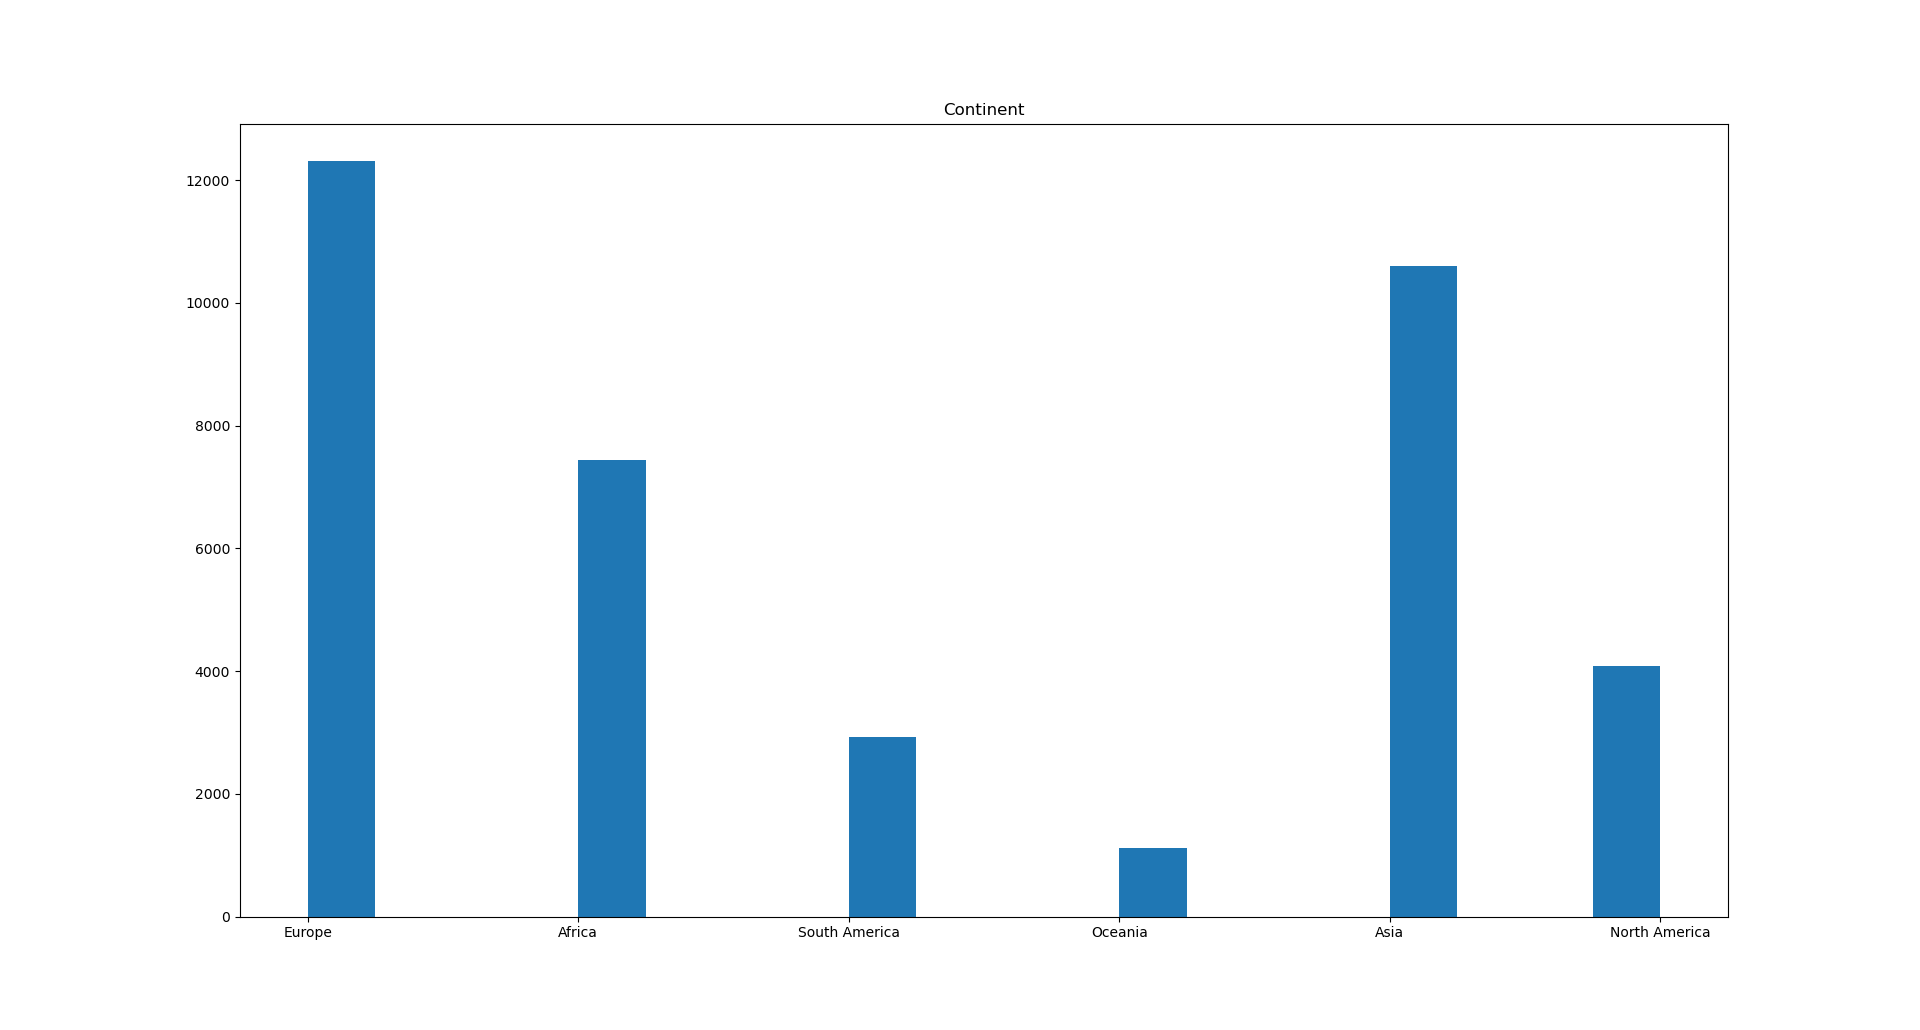
\includegraphics[width=\textwidth]{Figures/Question1/1. Histogram for Continent.png}
	\caption{Ιστόγραμμα για στήλη 'Continent'}
\end{figure}

\begin{figure}[H]
	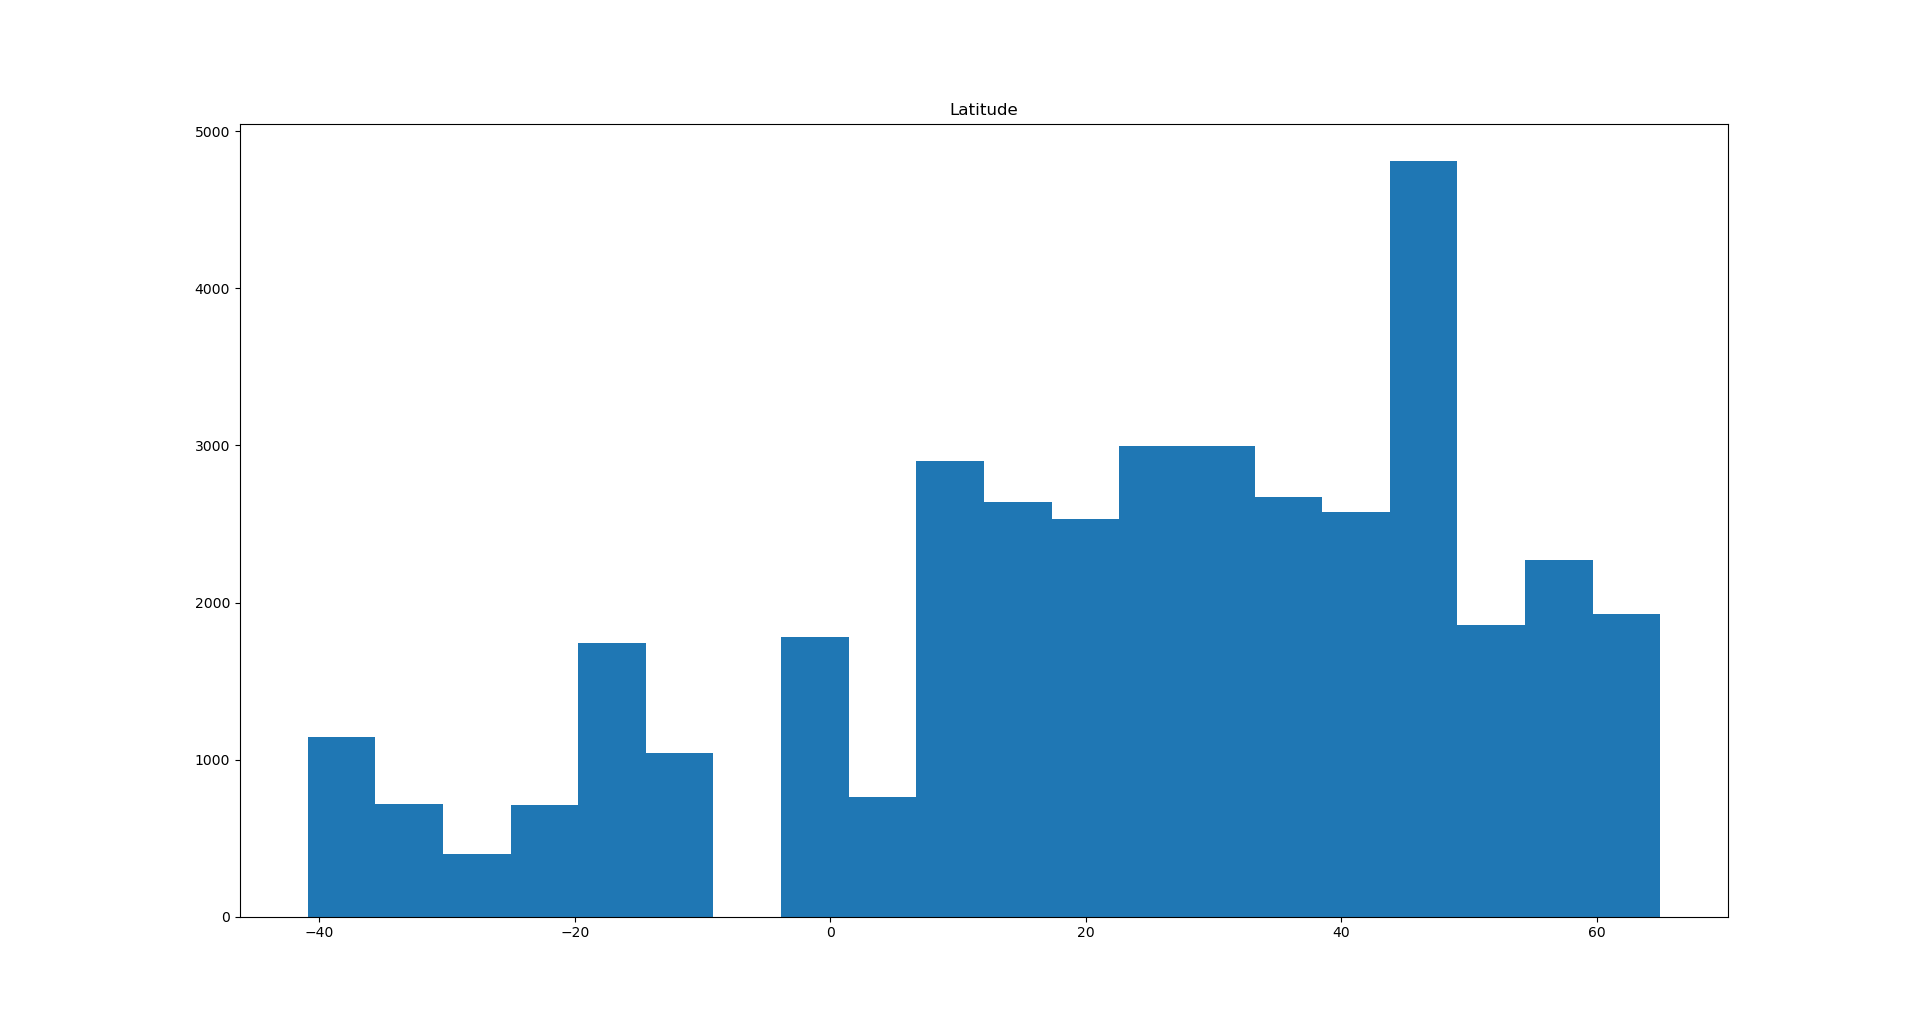
\includegraphics[width=\textwidth]{Figures/Question1/2. Histogram for Latitude.png}
	\caption{Ιστόγραμμα για στήλη 'Latitude'}
\end{figure}

\begin{figure}[H]
	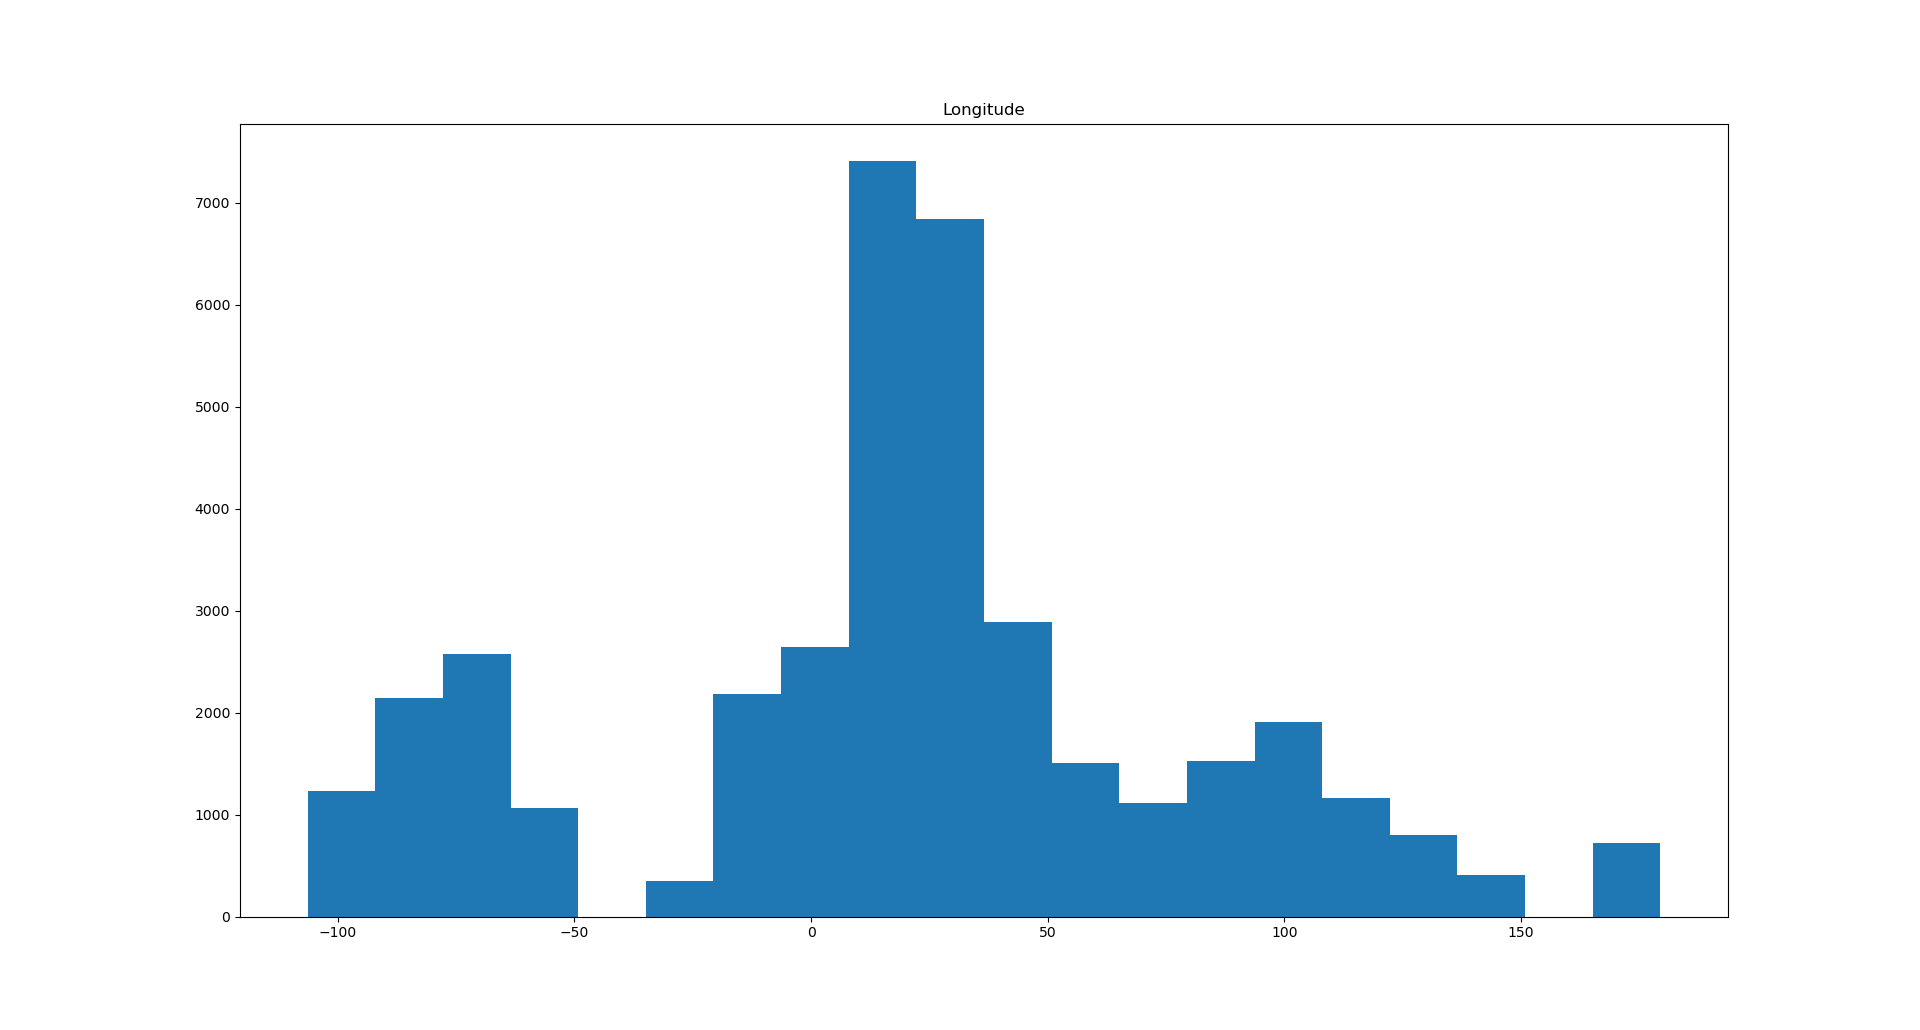
\includegraphics[width=\textwidth]{Figures/Question1/3. Histogram for Longtitude.png}
	\caption{Ιστόγραμμα για στήλη 'Longtitude'}
\end{figure}

\begin{figure}[H]
	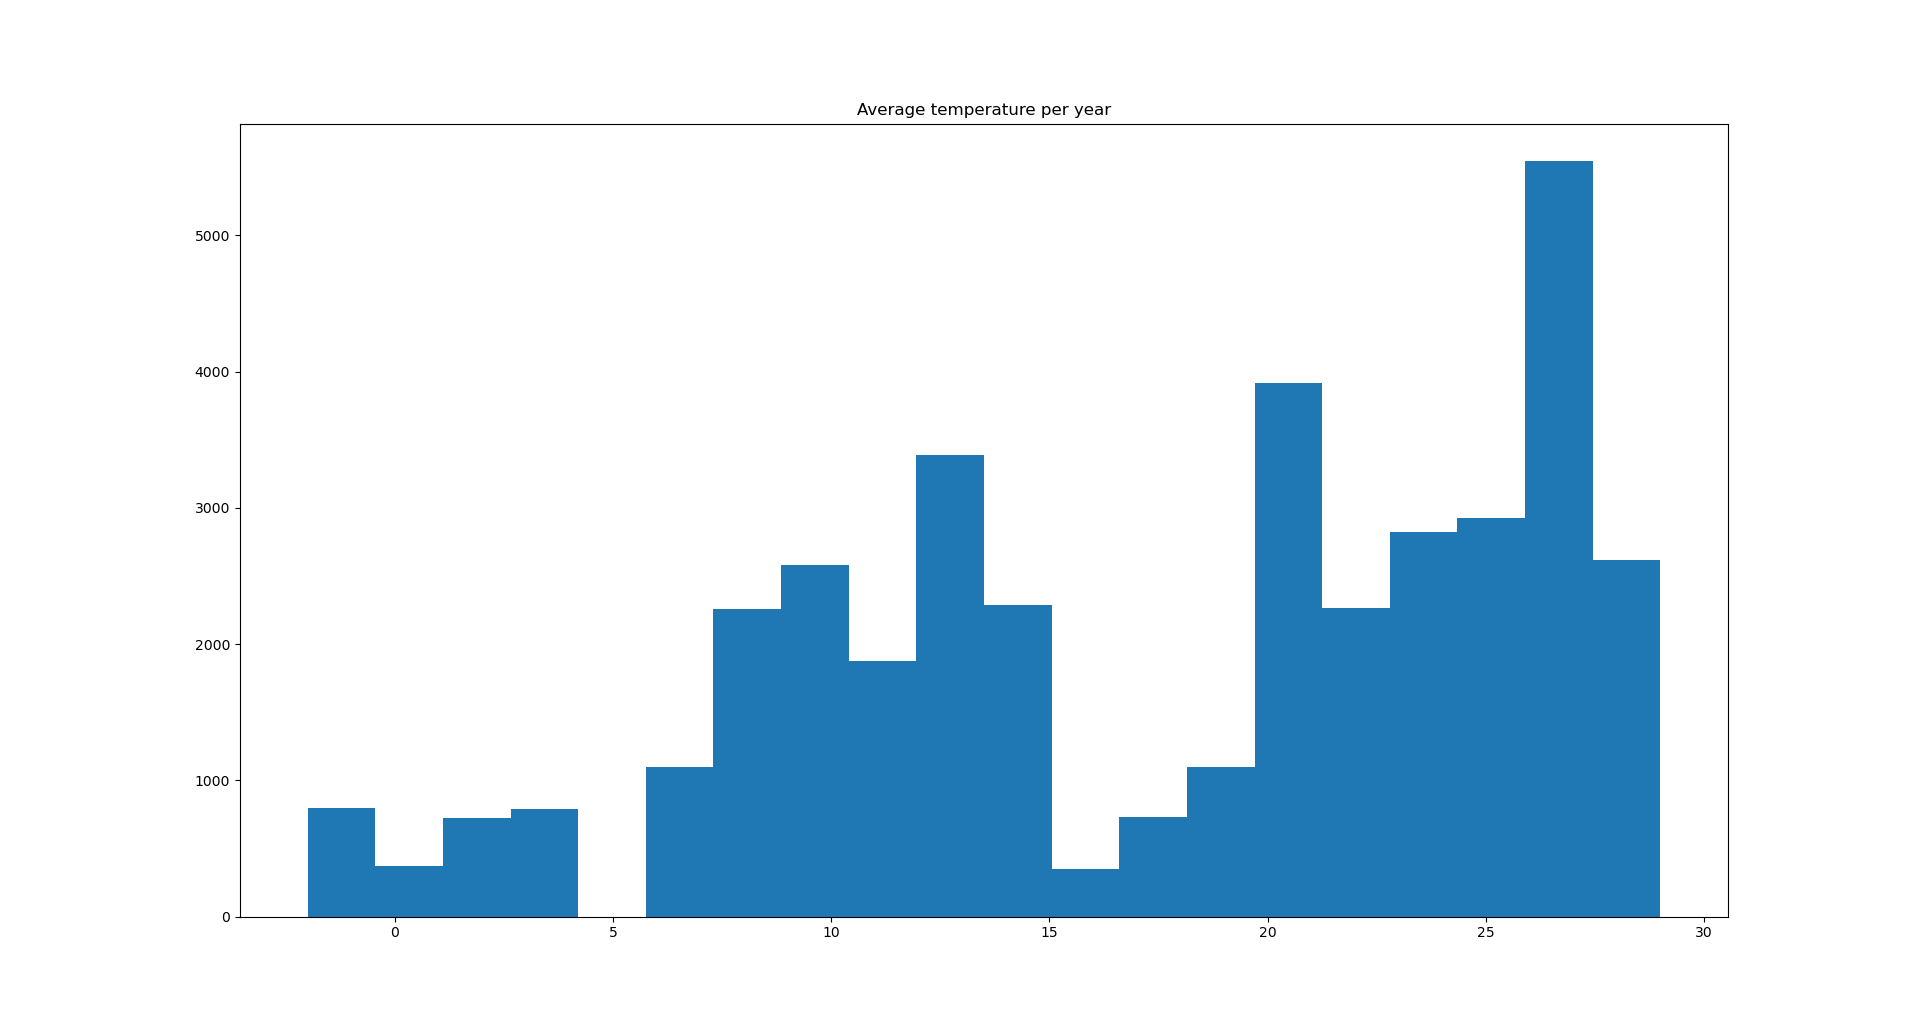
\includegraphics[width=\textwidth]{Figures/Question1/4. Histogram for average temperature per year.png}
	\caption{Ιστόγραμμα για στήλη 'Temperature'}
\end{figure}

\begin{figure}[H]
	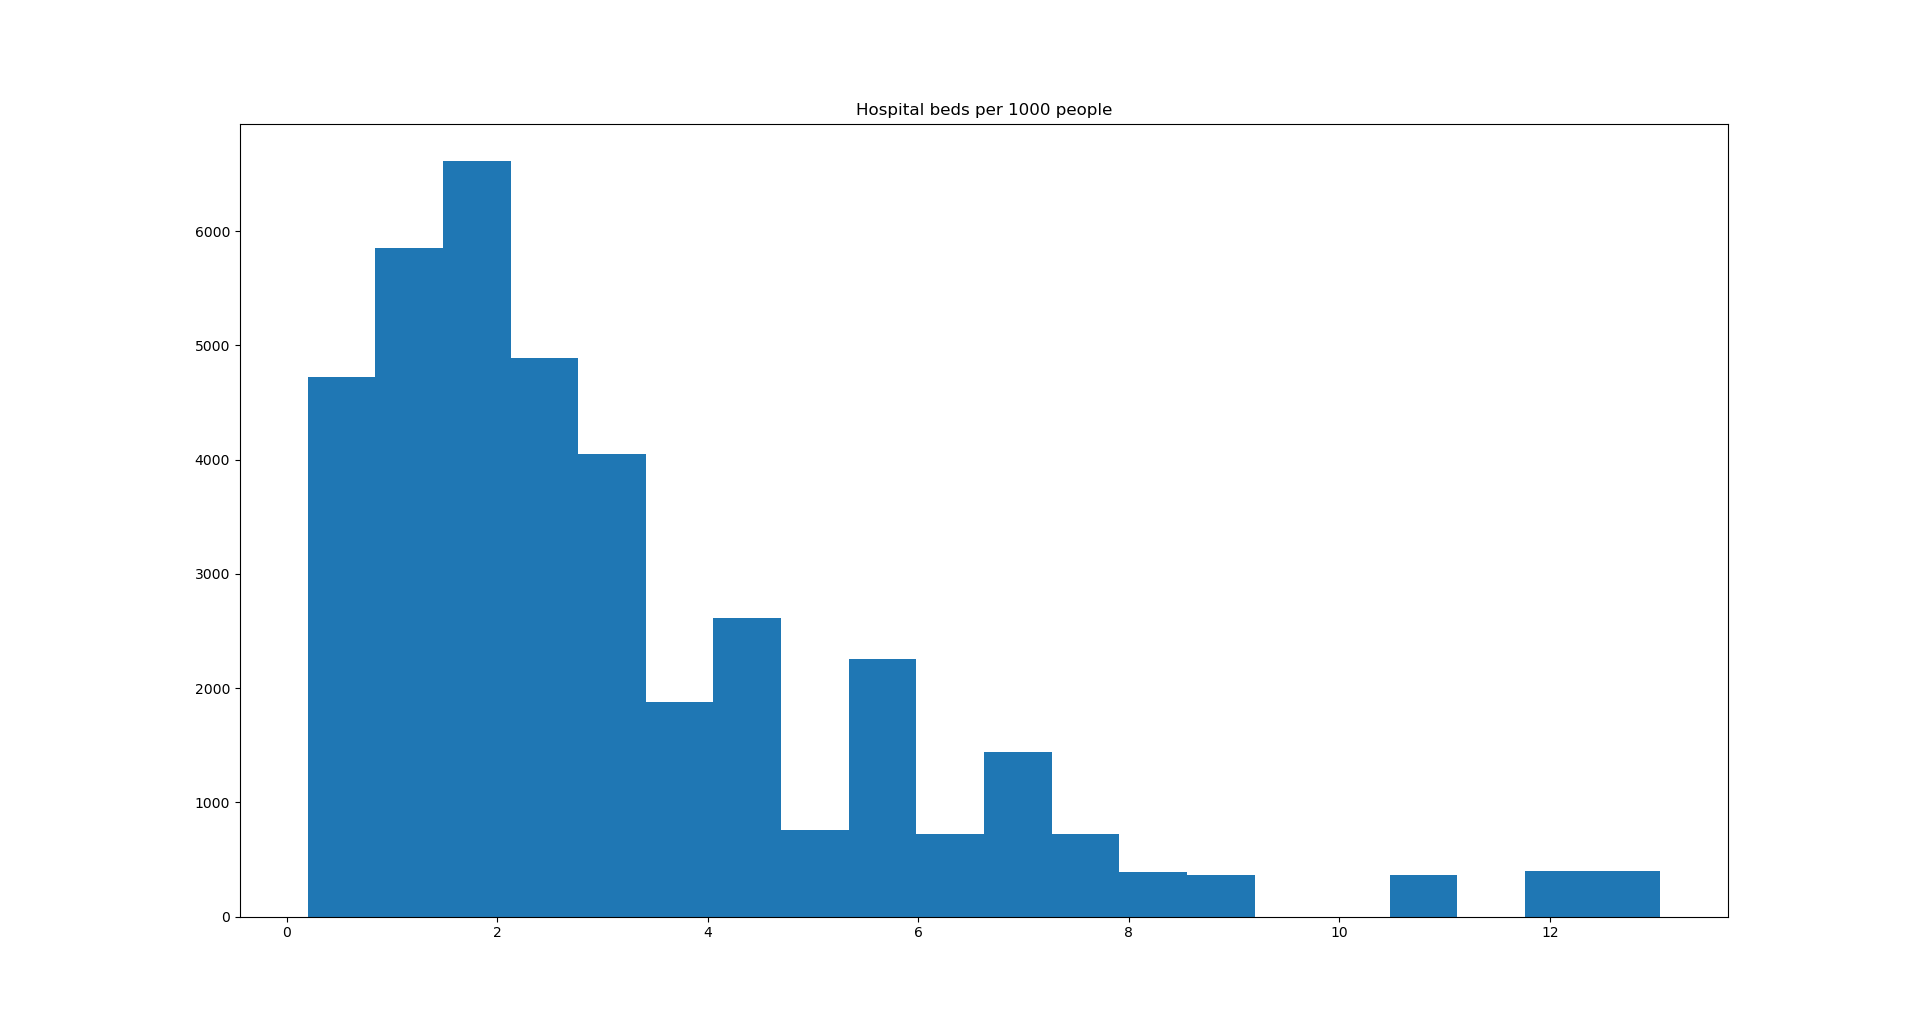
\includegraphics[width=\textwidth]{Figures/Question1/5. Histogram for hospital beds per 1000 people.png}
	\caption{Ιστόγραμμα για στήλη 'Hospital beds per 1000 people'}
\end{figure}

\begin{figure}[H]
	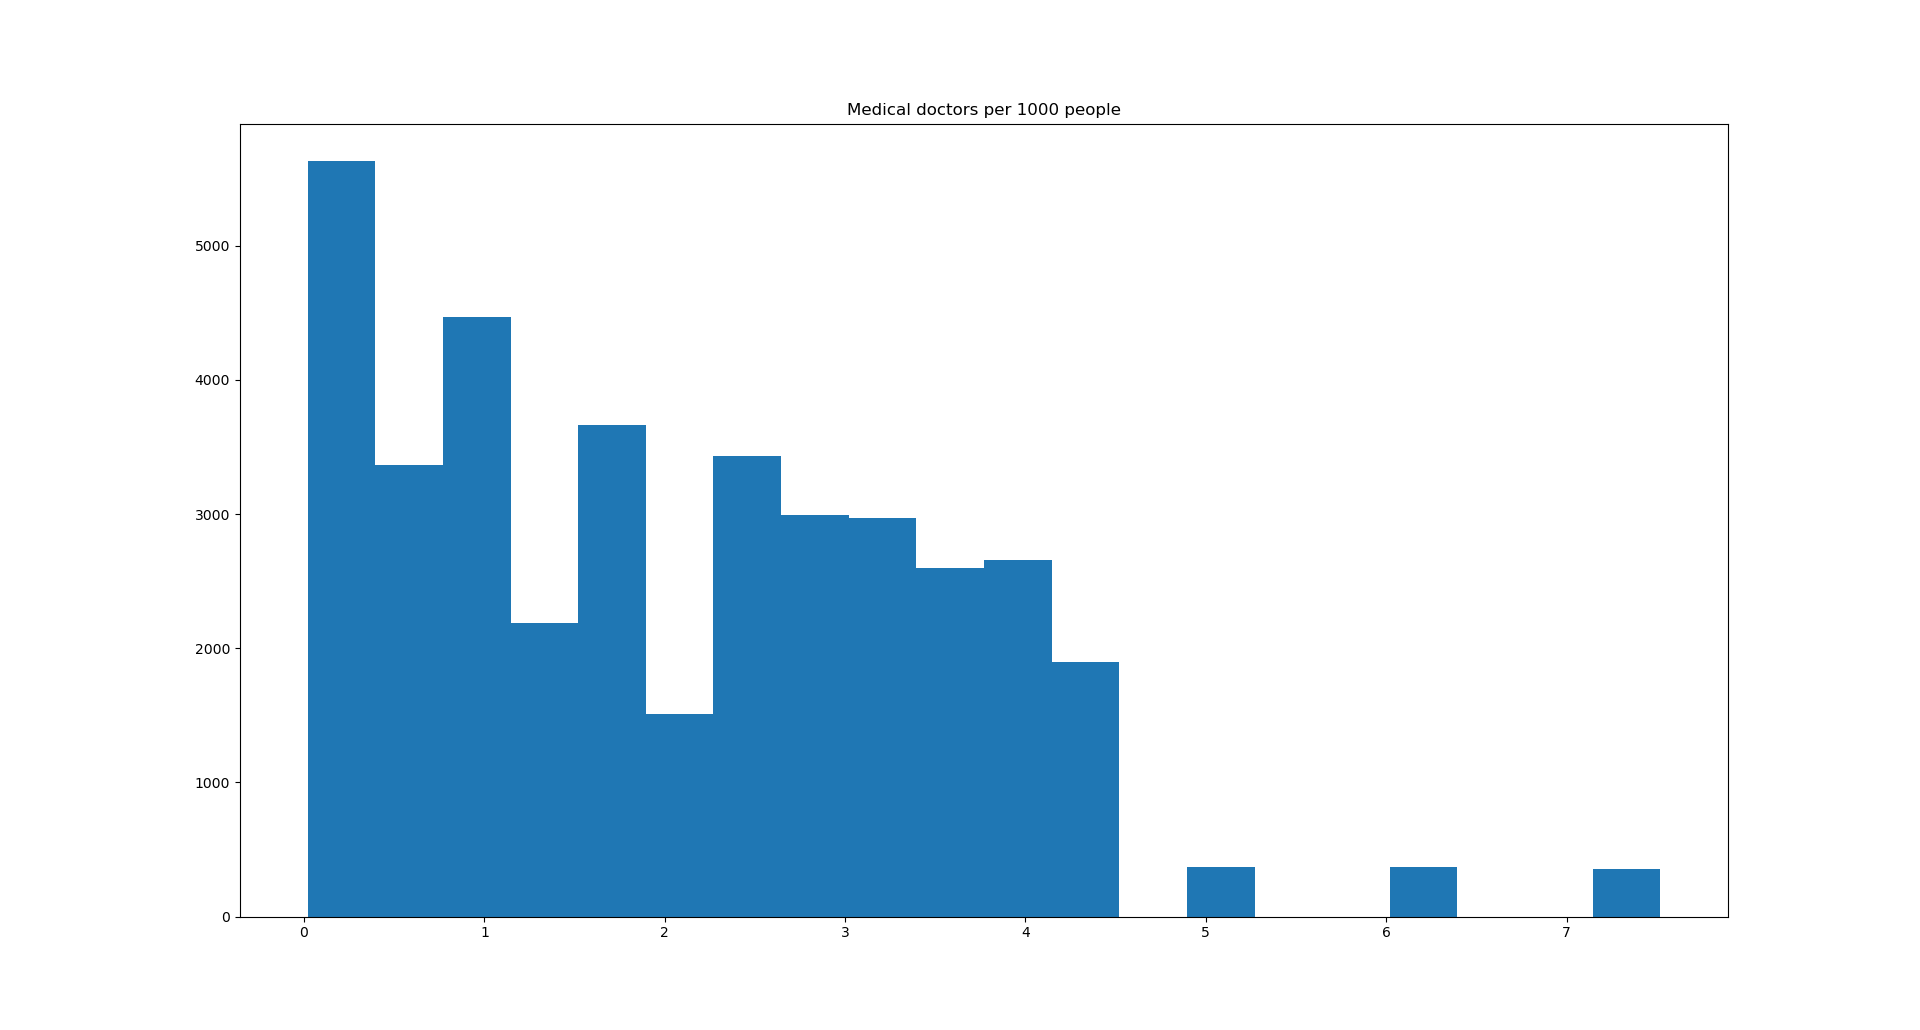
\includegraphics[width=\textwidth]{Figures/Question1/6. Histogram for medical doctors per 1000 people.png}
	\caption{Ιστόγραμμα για στήλη 'Medical doctors per 1000 people'}
\end{figure}

\begin{figure}[H]
	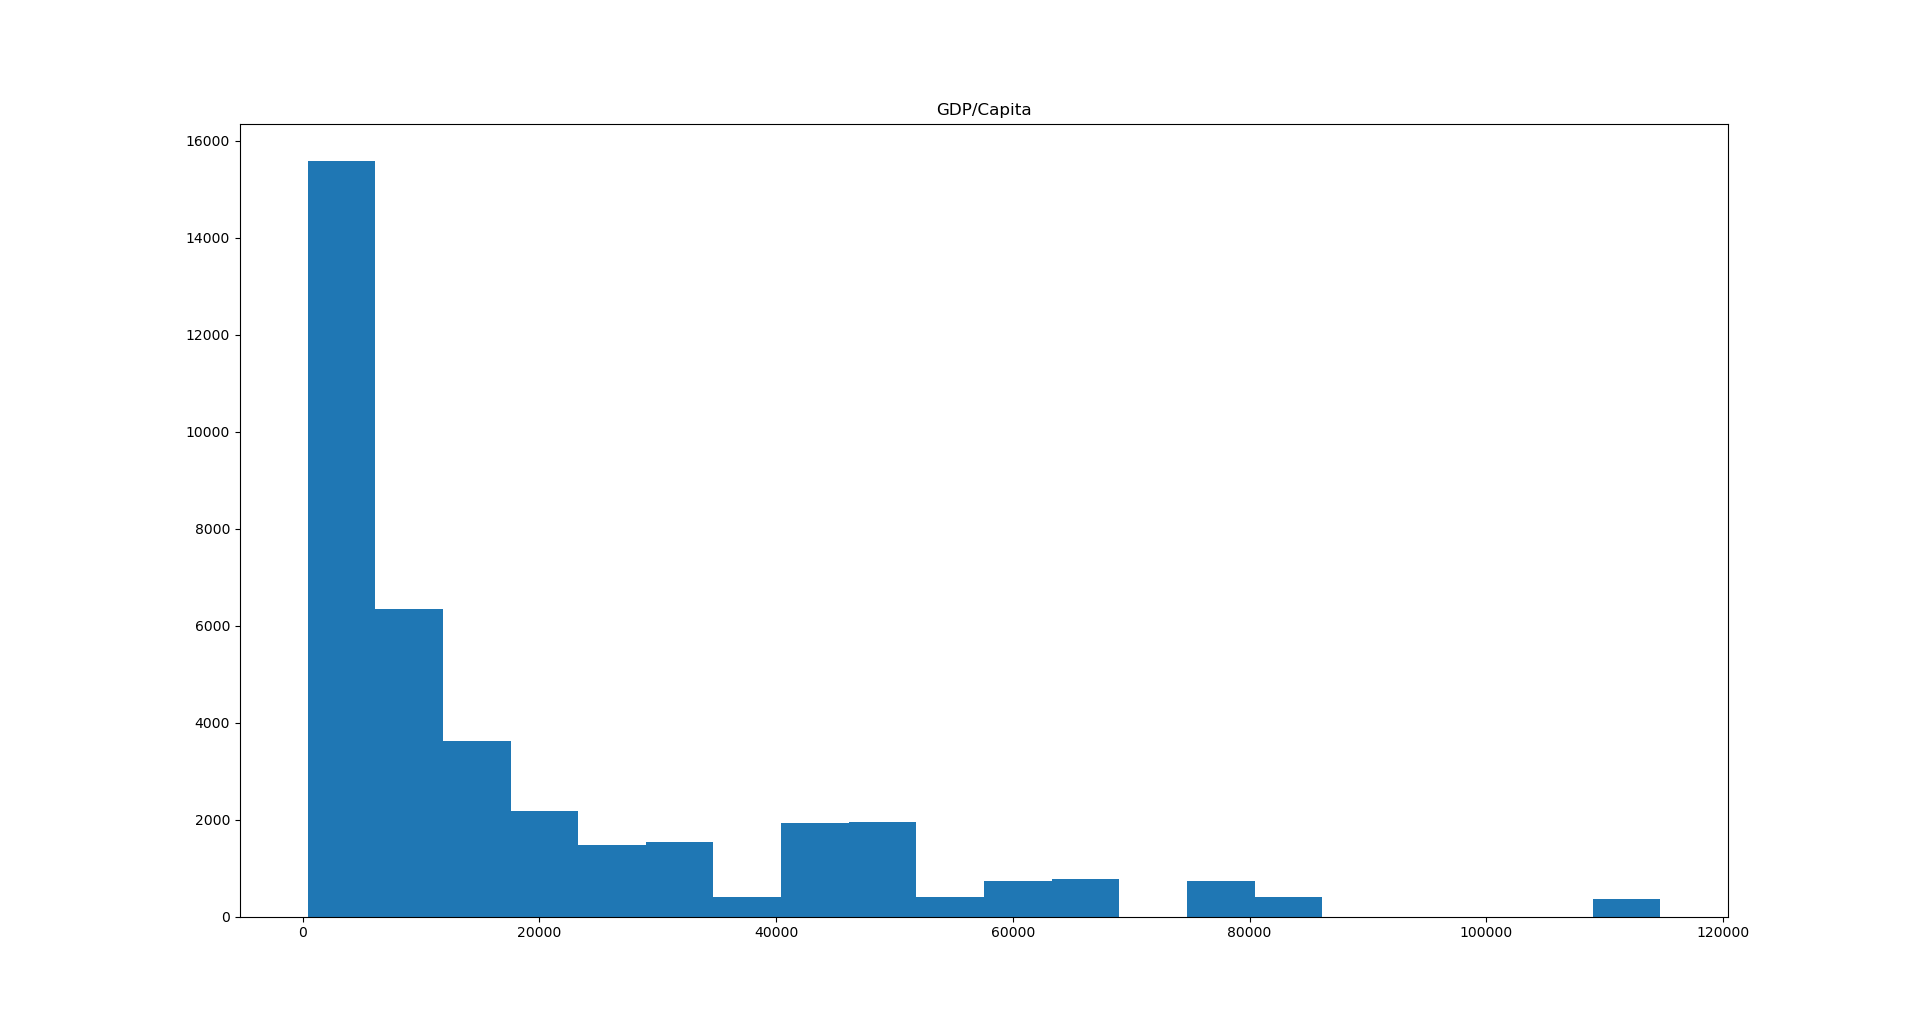
\includegraphics[width=\textwidth]{Figures/Question1/7. Histogram for GDP over capita.png}
	\caption{Ιστόγραμμα για στήλη 'GDP/Capita'}
\end{figure}

\begin{figure}[H]
	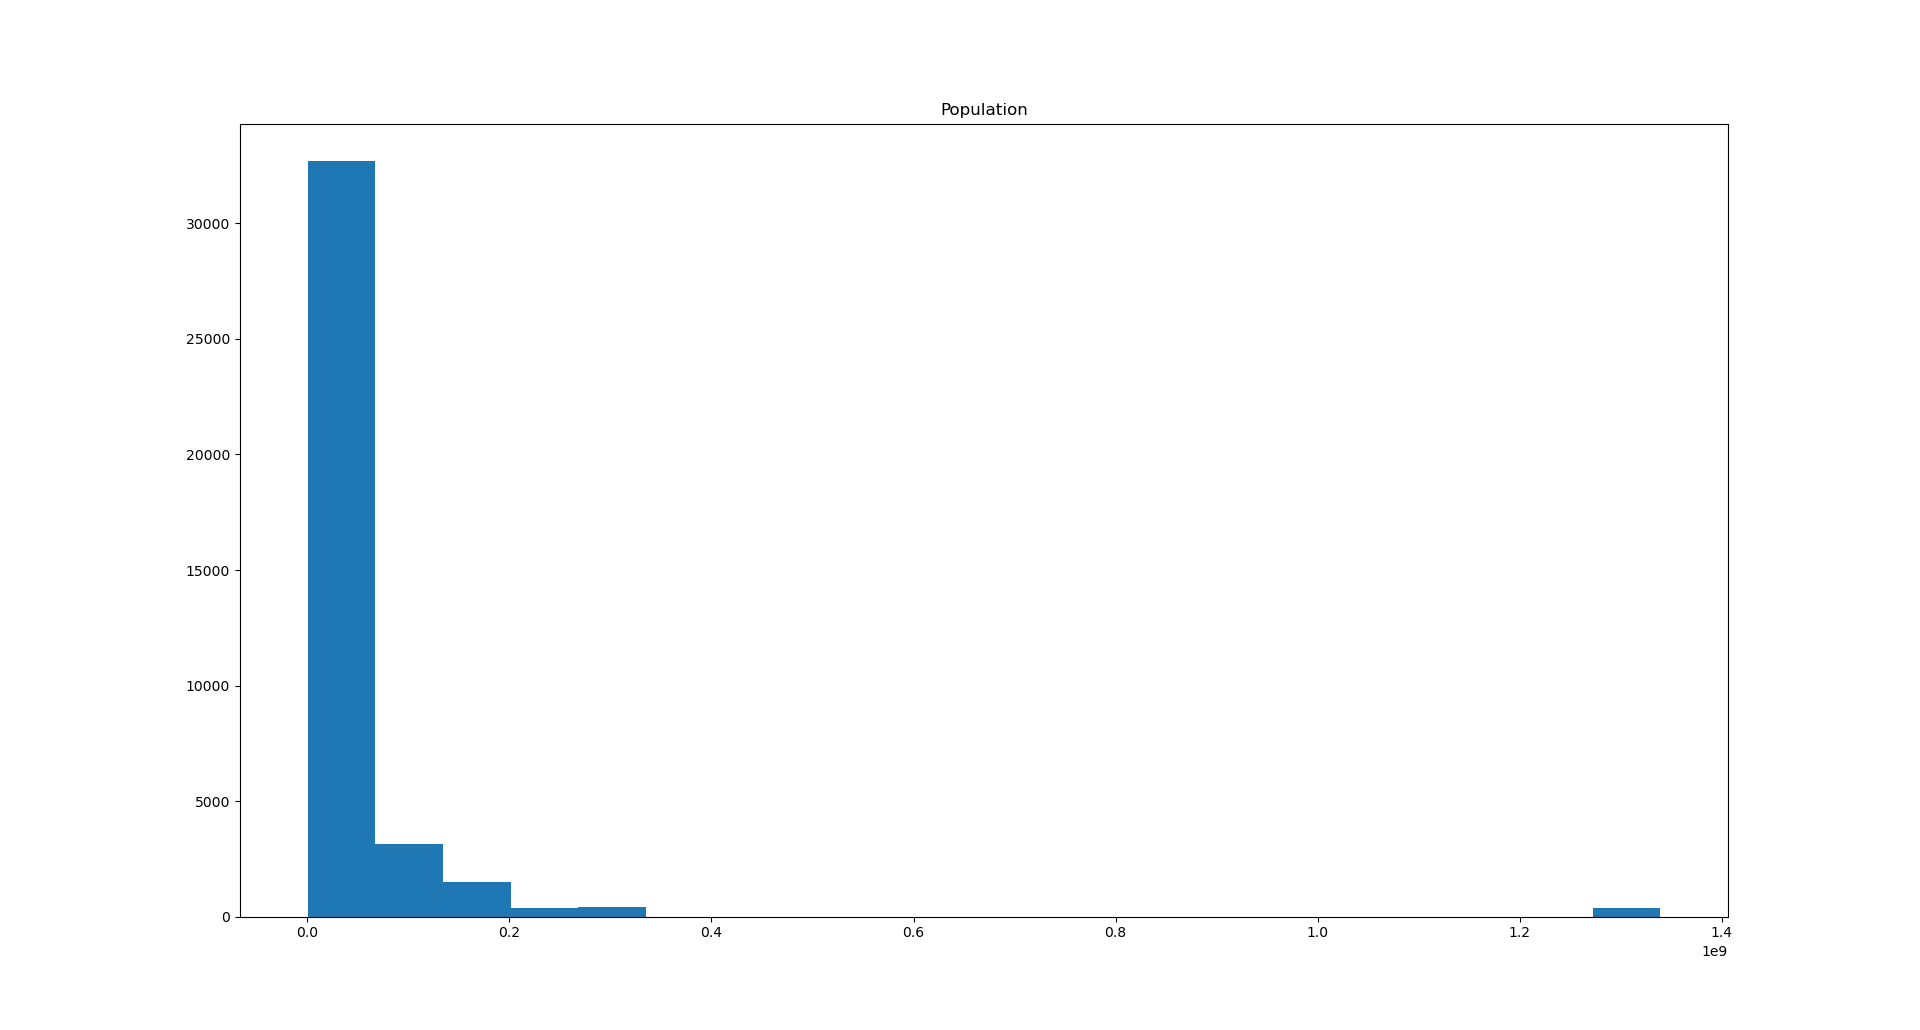
\includegraphics[width=\textwidth]{Figures/Question1/8. Histogram for population.png}
	\caption{Ιστόγραμμα για στήλη 'Population'}
\end{figure}

\begin{figure}[H]
	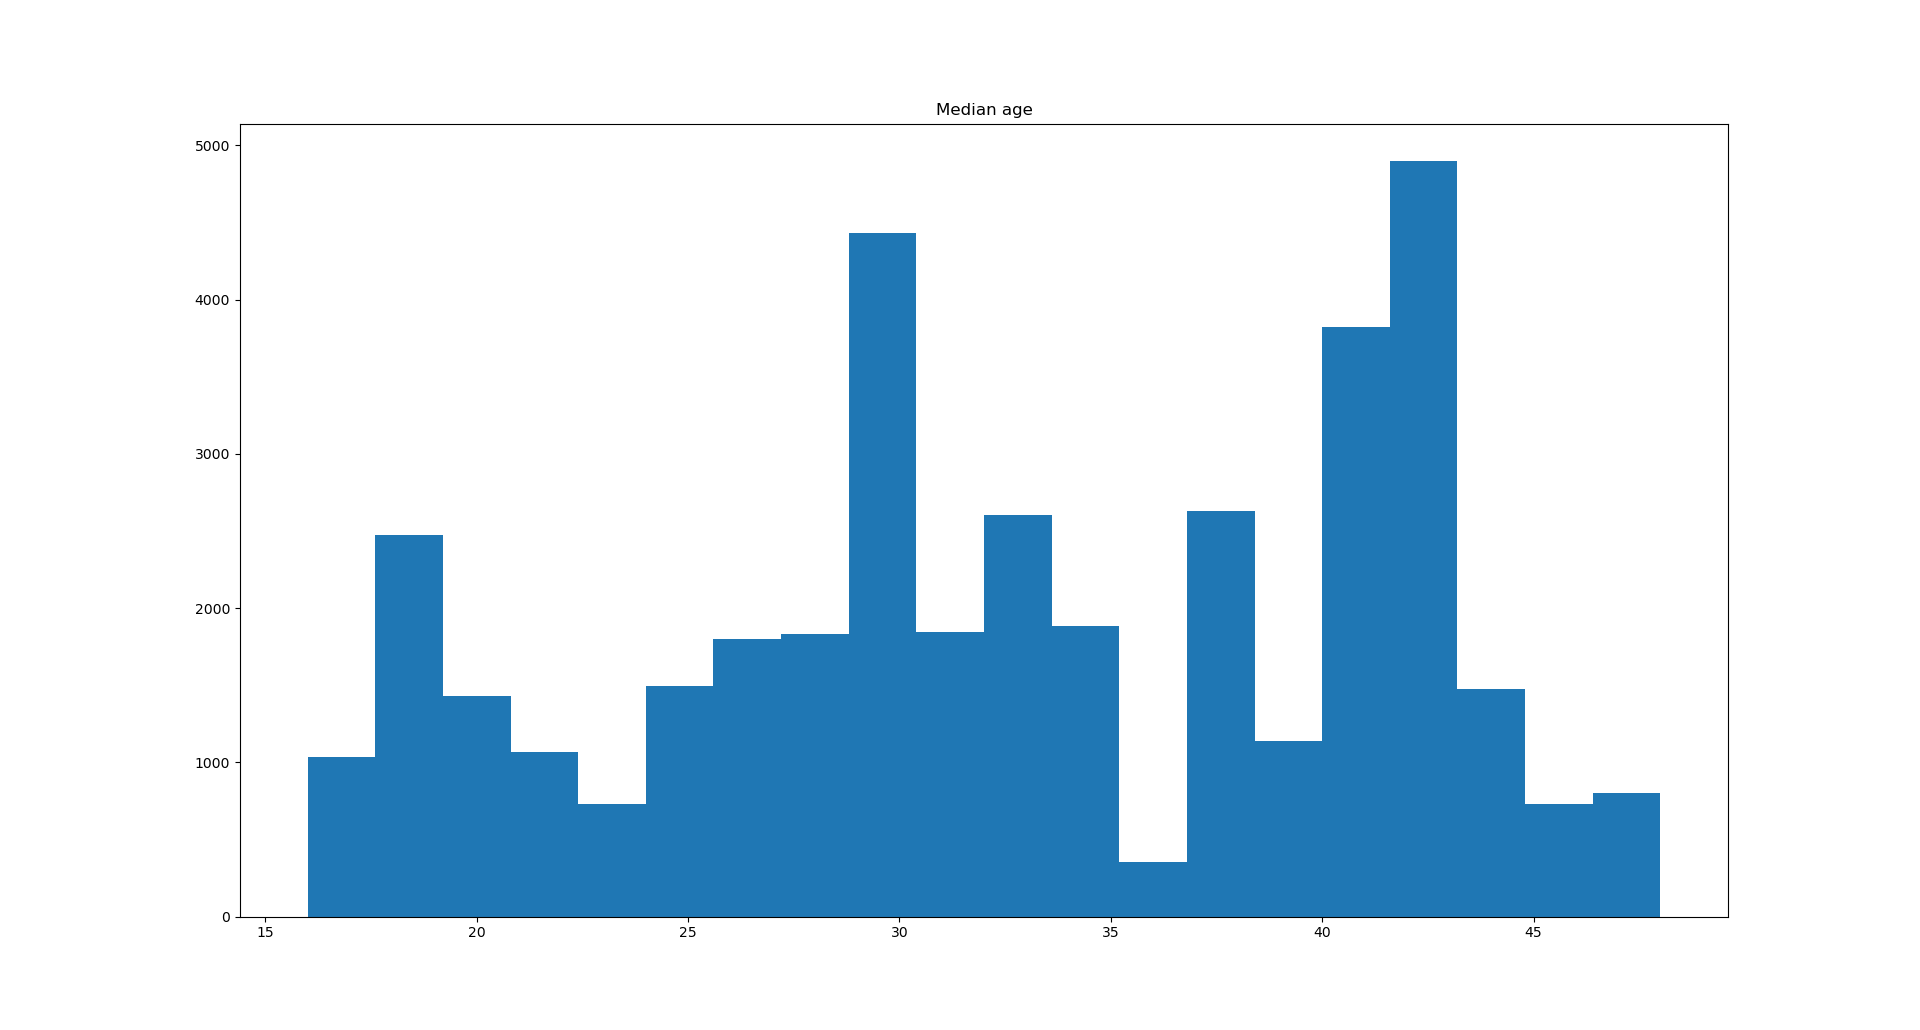
\includegraphics[width=\textwidth]{Figures/Question1/9. Histogram for median age.png}
	\caption{Ιστόγραμμα για στήλη 'Median age'}
\end{figure}

\begin{figure}[H]
	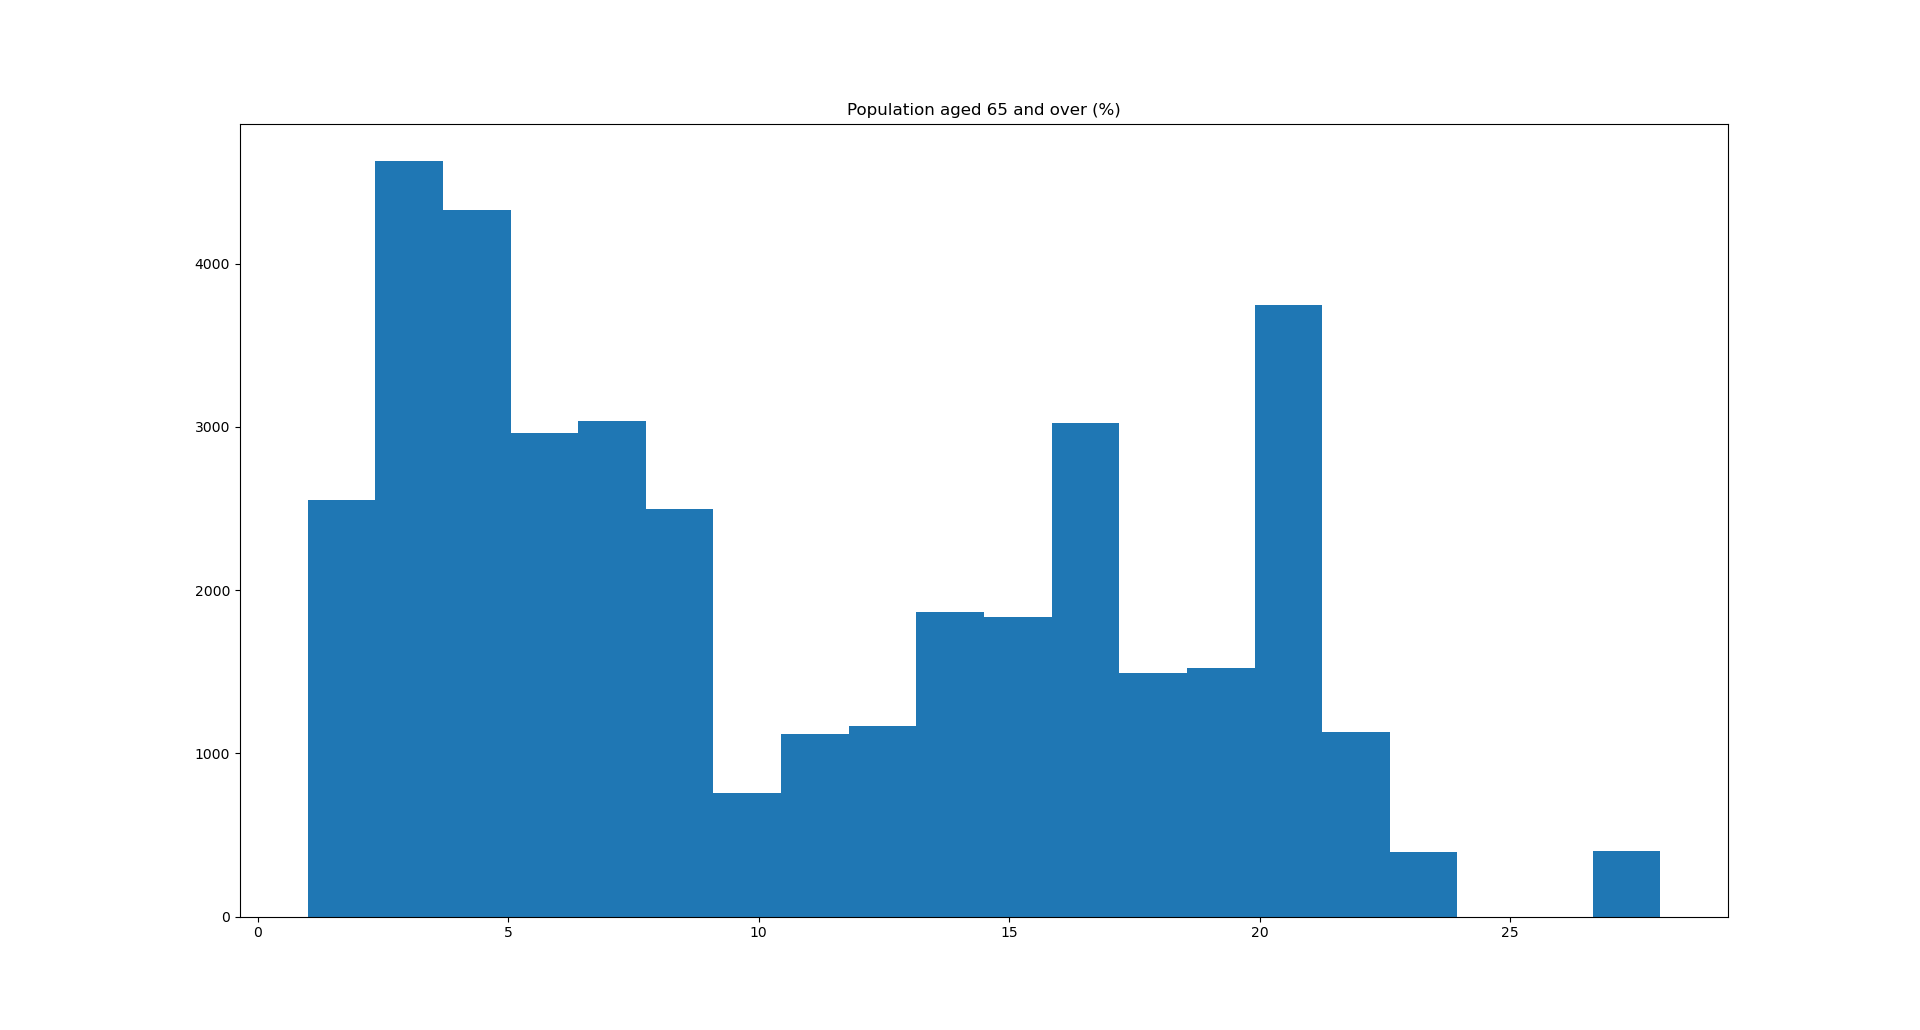
\includegraphics[width=\textwidth]{Figures/Question1/10. Histogram for population aged 65 and over.png}
	\caption{Ιστόγραμμα για στήλη 'Population aged 65 and over (\%)'}
\end{figure}

\begin{figure}[H]
	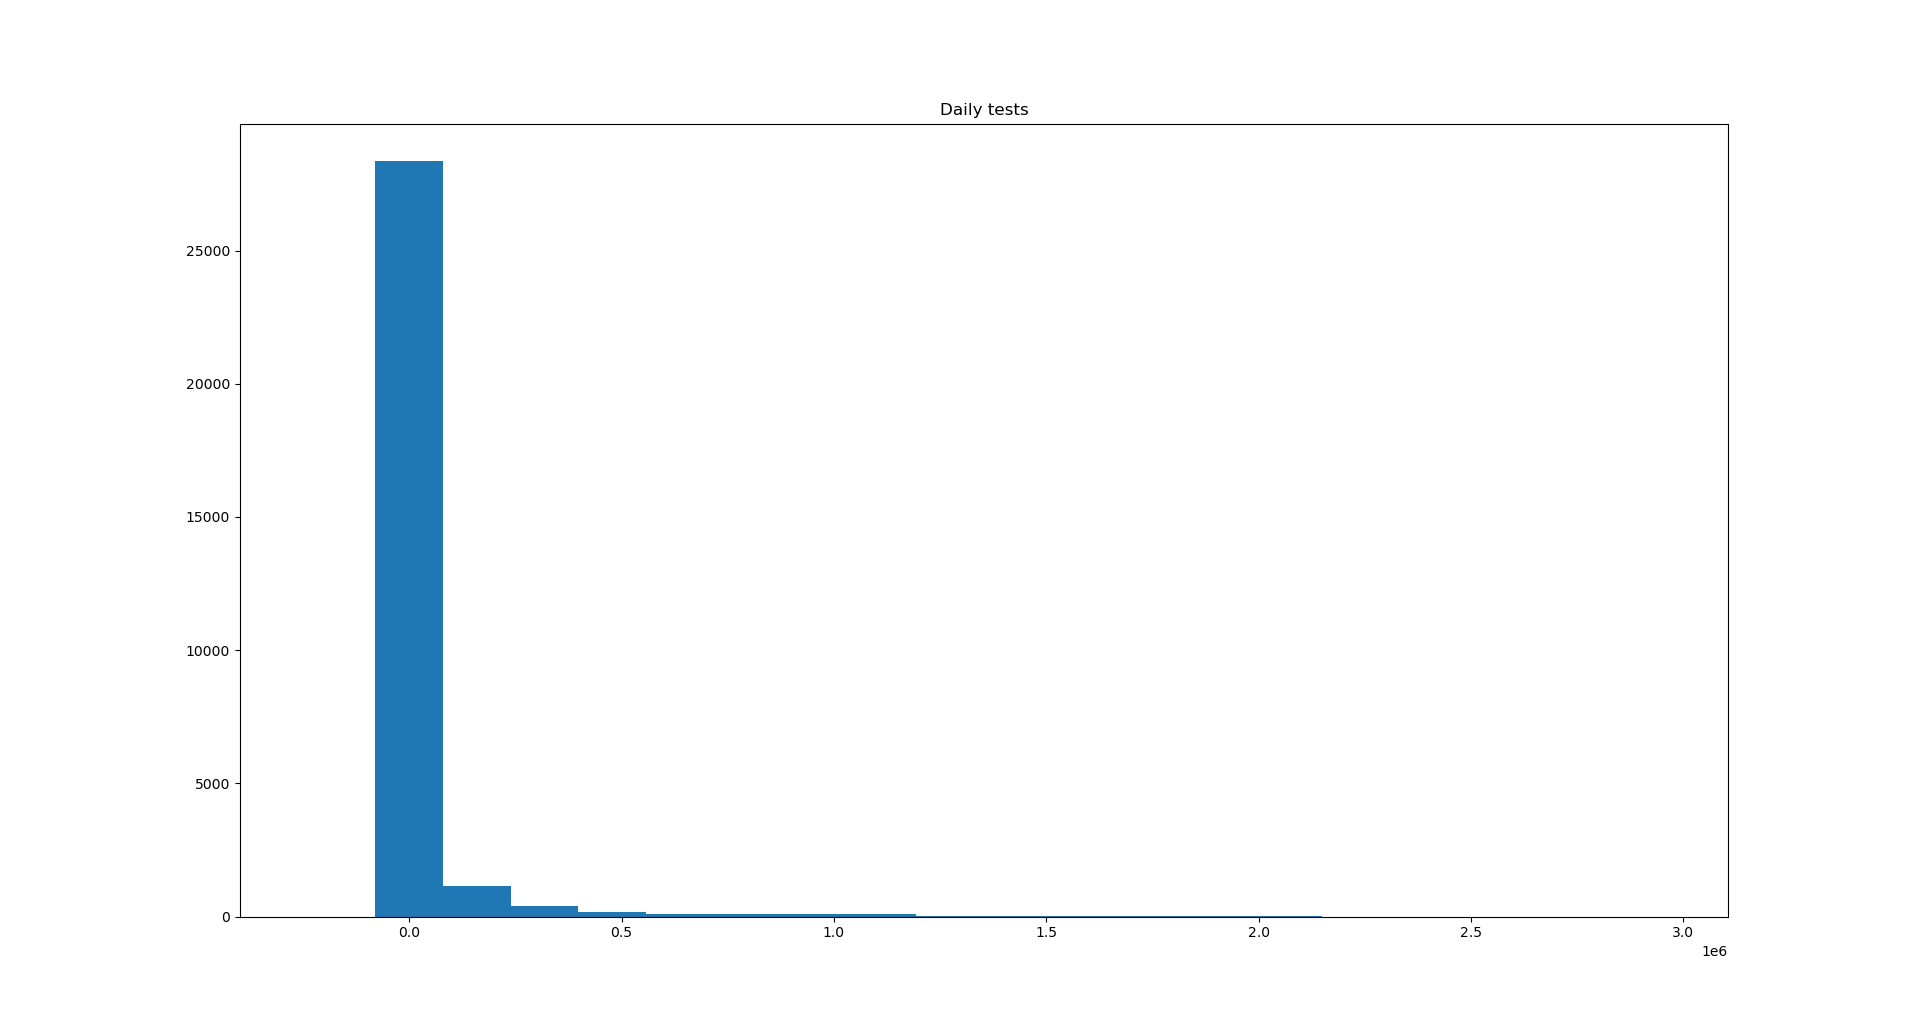
\includegraphics[width=\textwidth]{Figures/Question1/11. Histogram for daily tests.png}
	\caption{Ιστόγραμμα για στήλη 'Daily tests'}
\end{figure}

\begin{figure}[H]
	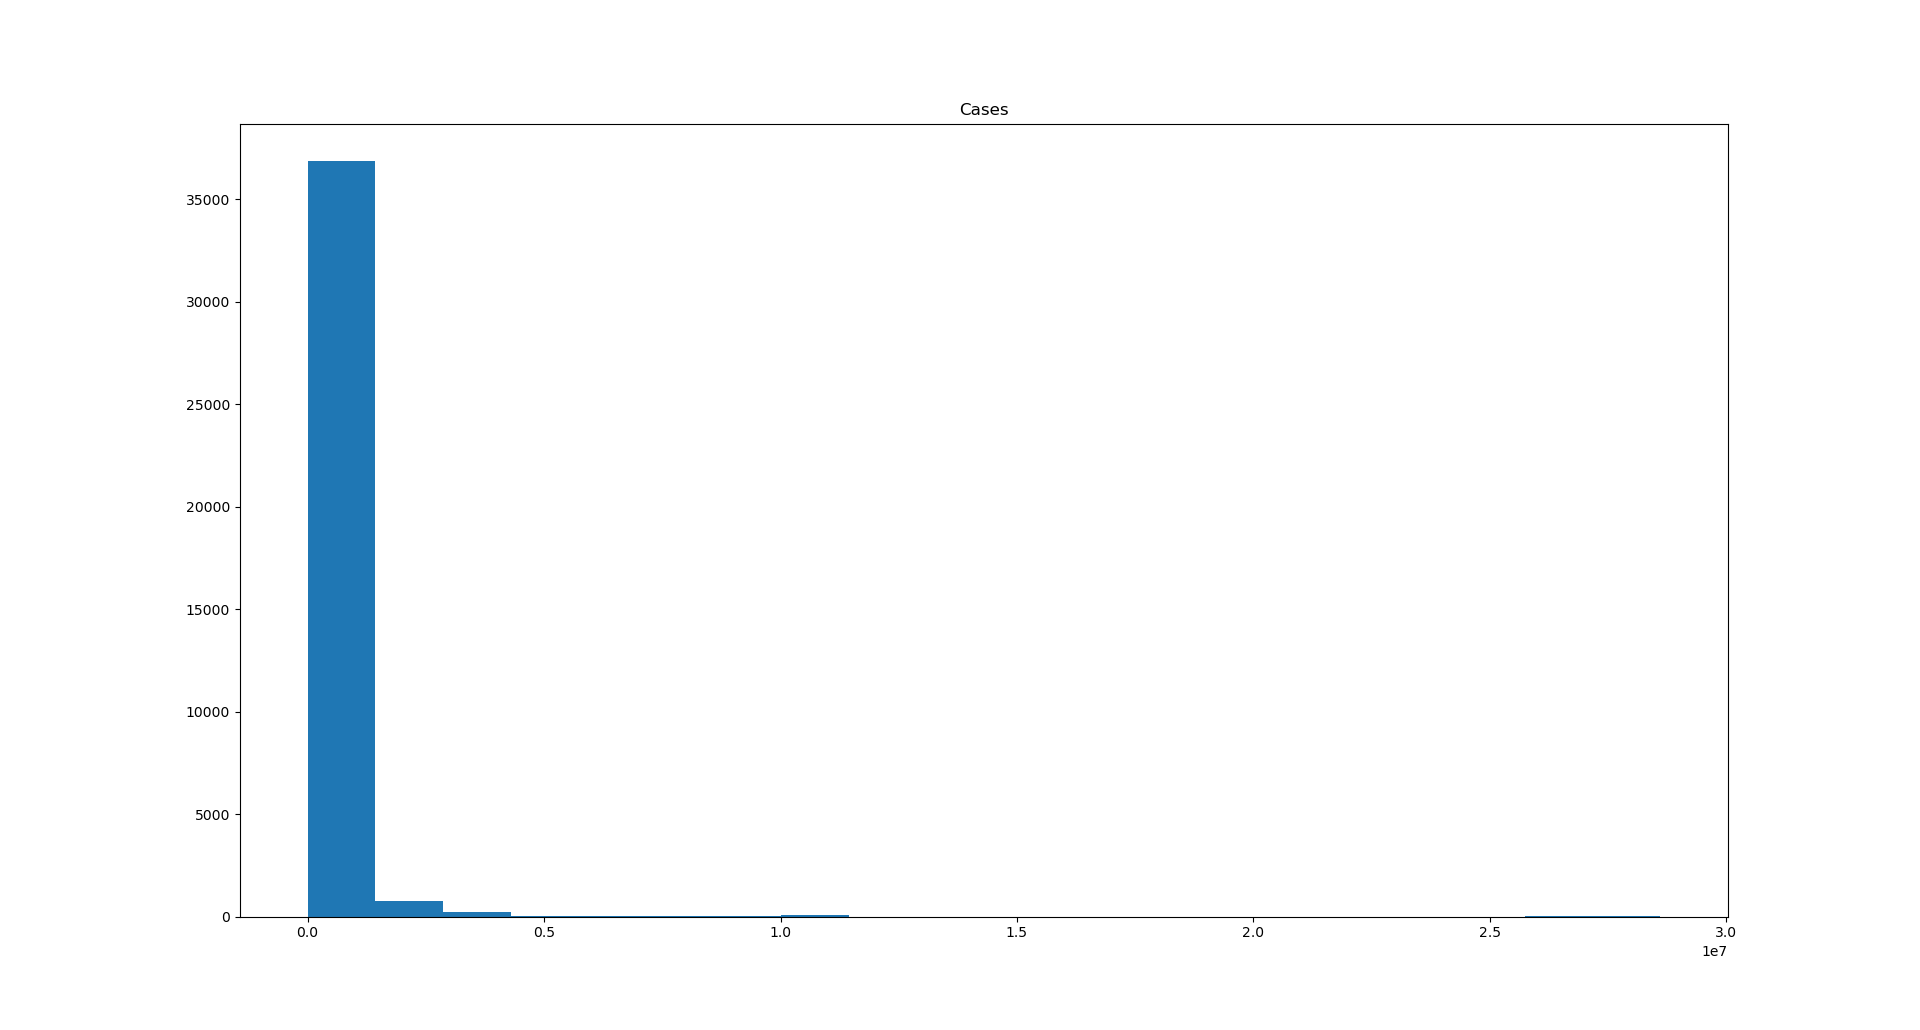
\includegraphics[width=\textwidth]{Figures/Question1/12. Histogram for cases.png}
	\caption{Ιστόγραμμα για στήλη 'Cases'}
\end{figure}

\begin{figure}[H]
	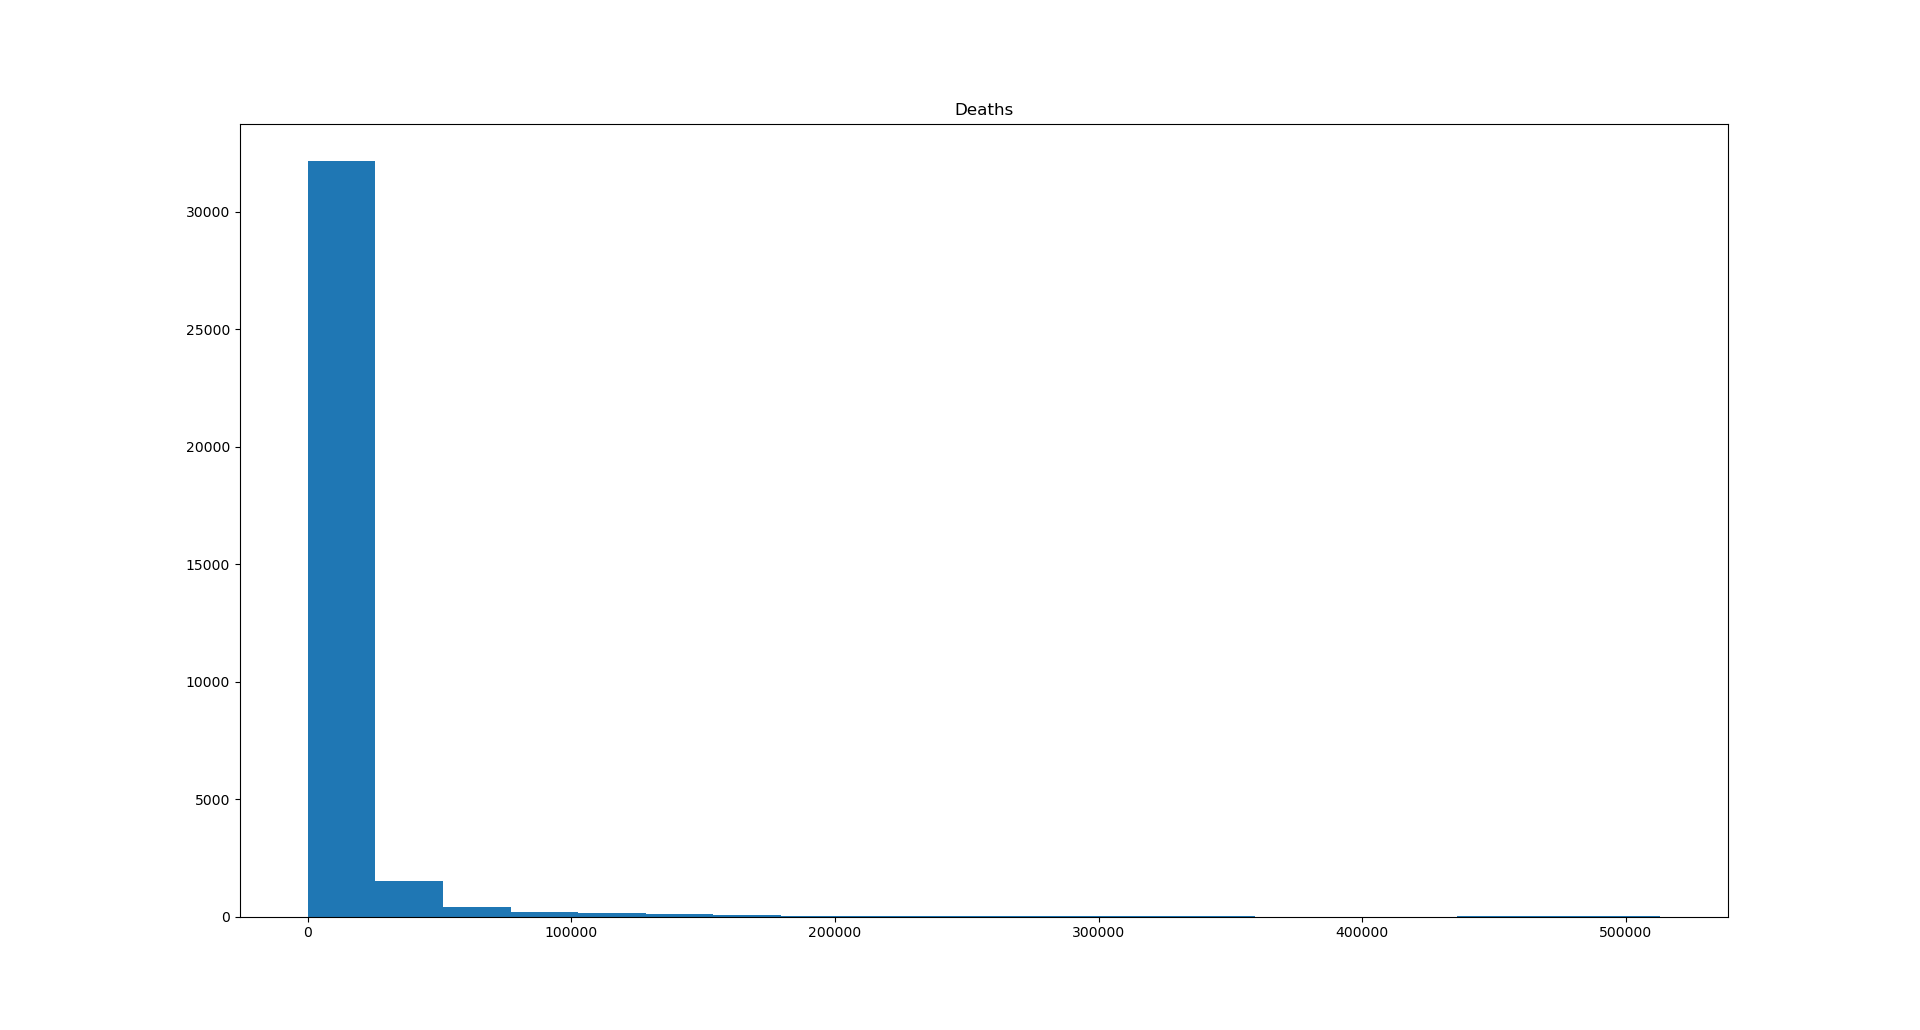
\includegraphics[width=\textwidth]{Figures/Question1/13. Histogram for deaths.png}
	\caption{Ιστόγραμμα για στήλη 'Deaths'}
\end{figure}

Τέλος παρακάτω παρουσιάζουμε το Correlation Matrix Heatmap που φτιάξαμε για τις στήλες του dataset.

\begin{figure}[H]
	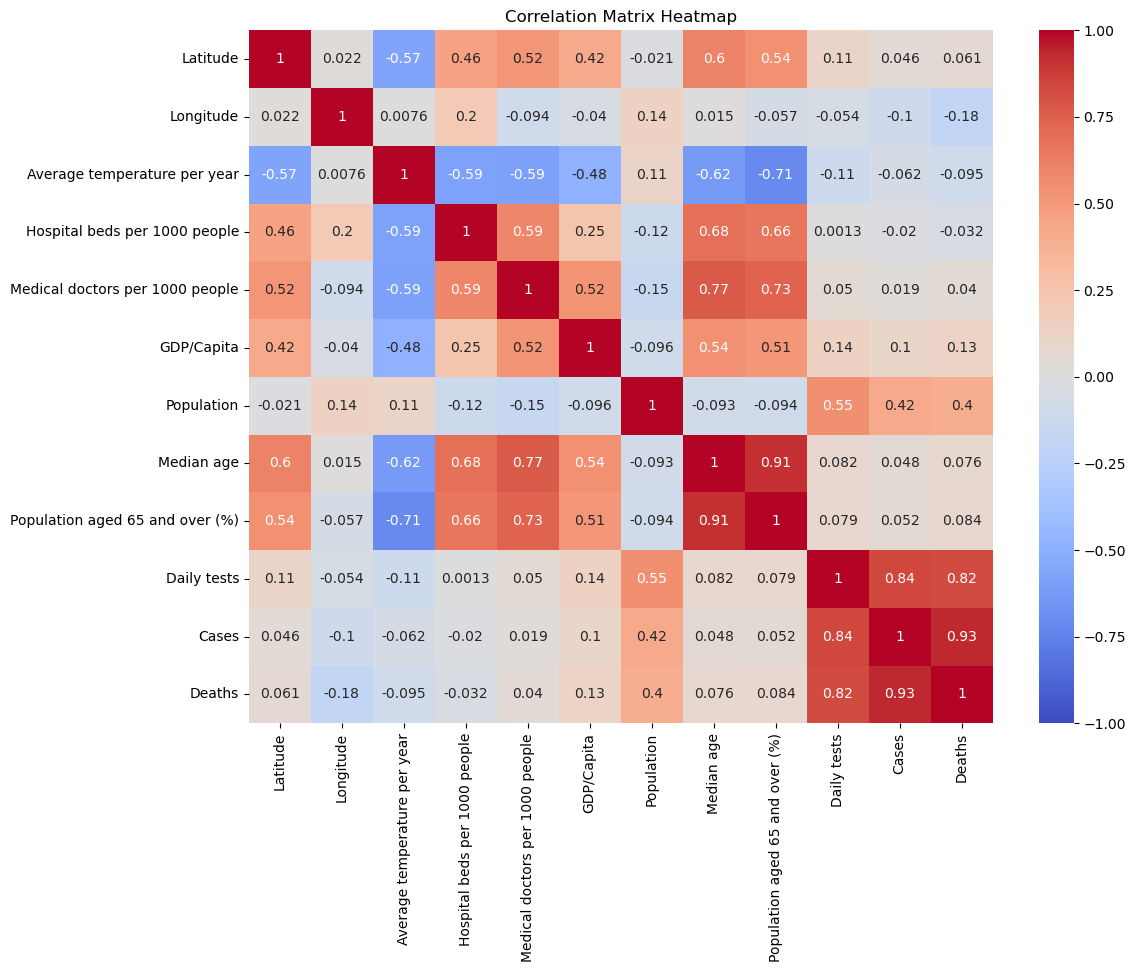
\includegraphics[width=\textwidth]{Figures/Question1/14. Correlation matrix heatmap.png}
	\caption{Correlation Matrix Heatmap για τις στήλες}
\end{figure}

\subsubsection{Συμπεράσματα}

Από τα στατιστικά στοιχεία και τα ιστογράμματα συμπεραίνουμε πως πολλές από τις στήλες περιέχουν στοιχεία που φαίνεται να αποτελούν half-normal κατανομές, με διαφορετικές τιμές μέσης τιμής και διασποράς. Οι στήλες αυτές είναι οι 'Medical doctors per 1000 people', 'GDP/Capita', 'Population', 'Daily tests', 'Cases', 'Deaths'. Επίσης η στήλη 'Hospital beds per 1000 people' φαίνεται να ακολουθεί log-normal κατανομή. Για τις υπόλοιπες στήλες δεν μπορούμε να συμπεράνουμε ότι ανήκουν σε κάποια κατανομή.

Από το Correlation Matrix Heatmap παρατηρούμε ότι υπάρχει μεγάλη συσχέτιση μεταξύ 'Daily tests', 'Cases' και 'Deaths', καθώς και μεταξύ 'Median age', 'People aged 65 and over (\%)', 'Hospital beds per 1000 people' και 'Medical doctors per 1000 people'. Υπάρχει επίσης μεγάλη αρνητική συσχέτιση μεταξύ του 'Average Temperature per year' σε σχέση με τα 'Population aged 65 and over (\%)', 'Median age', 'Medical doctors per 1000 people', 'Hospital beds per 1000 people' και 'Latitude'. Σημειώνουμε ότι υπάρχουν και άλλες συσχετίσεις εκτός από αυτές που αναφέρονται, αλλά δεν είναι τόσο ισχυρές όσο αυτές που αναφέρουμε εδώ, οπότε τις παραλείπουμε για λόγους συντομίας, εφόσον φαίνονται και στο heatmap.

\section{Υλοποίηση και Αποτελέσματα Ερωτήματος 2}

\subsection{Σύντομη Περιγραφή της Διαδικασίας Υλοποίησης}

\subsubsection{Χειρισμός Τιμών που Λείπουν}

Για την υλοποίηση του ερωτήματος αυτού, αρχικά αφού διαβάσουμε το αρχείο του dataset θα πρέπει να αντιμετωπίσουμε τις τιμές που λείπουν από αυτό. Αυτό το επιτυγχάνουμε με τη χρήση των εντολών:

\begin{lstlisting}[language=Python]
df = df.groupby('Entity',group_keys=False).apply(lambda x: x.fillna(method='ffill'))
df = df.groupby('Entity',group_keys=False).apply(lambda x: x.fillna(method='bfill'))
\end{lstlisting}

Αυτές οι εντολές επιτυγχάνουν αρχικά το grouping του DataFrame με βάση το 'Entity' (χώρα) και μετά την εφαρμογή της fillna μεθόδου, η οποία συμπληρώνει τις τιμές που λείπουν αρχικά με χρήση forward fill στη πρώτη εντολή και έπειτα με backward fill στη δεύτερη εντολή.

Το forward fill επιτυγχάνει την αντικατάσταση τιμών που λείπουν με την τελευταία προηγούμενη καταγεγραμμένη τιμή, αλλά επειδή γίνεται να υπάρχουν ακόμα κενά (πχ αν λείπουν τιμές στην αρχή των καταγεγραμμένων στοιχείων), κάνουμε έπειτα το backward fill που συμπληρώνει τιμές που λείπουν με την επόμενη καταγεγραμμένη τιμή.

Ο λόγος που προτιμούμε πρώτα να κάνουμε forward fill και μετά backward fill είναι επειδή με αυτόν τον τρόπο ελαχιστοποιούμε την συμπλήρωση με βάση τις μελλοντικές ως προς τη χρονική στιγμή που συμπληρώνουμε τιμές.

Έπειτα αφαιρούμε όλα τα duplicates που τυχόν προέκυψαν με χρήση της μεθόδου drop\_duplicates() του Pandas.

\subsubsection{Δημιουργία Νέων Πεδίων και Επιλογή Πεδίων για το Clustering}

Αποφασίσαμε για το πιο αποτελεσματικό clustering να προσθέσουμε ορισμένα πεδία στα δεδομένα τα οποία εξάγονται από τα υπόλοιπα δεδομένα. Πιο συγκεκριμένα τα νέα πεδία αυτά τα ορίζουμε ως εξής:

\begin{itemize}
    \item Positive Ratio = Today's New Cases / Daily Tests
    \item Death Ratio = Total Deaths / Total Cases
    \item Tested Ratio = Daily Tests / Population
\end{itemize}

Αποφασίσαμε επίσης να χρησιμοποιήσουμε όλα τα πεδία των δεδομένων για το clustering, εκτός από τις ημερομηνίες (επειδή θα κάνουμε aggregation, όπως εξηγείται παρακάτω). Ενώ η εκφώνηση μας ζητάει να χωρίσουμε τις συστάδες με βάση τις επιδόσεις τους στην αντιμετώπιση του ίου, πιστεύουμε πως στοιχεία όπως τις γεωγραφικές συντεταγμένες, η ήπειρος, η μέση θερμοκρασία και το GDP/Capita παρουσιάζουν έμμεση πληροφορία για την αντιμετώπιση του ίου, εφόσον κοντινές χώρες έχουν συνήθως μεγαλύτερες ανταλλαγές πληθυσμών και παρόμοια οικονομική κατάσταση, το οποίο επηρεάζει την δυνατότητα της χώρας να αντιμετωπίσει αποτελεσματικά τον ιό. Επίσης και η μέση θερμοκρασία μπορεί αν επηρεάσει το ανοσοποιητικό σύστημα των πολιτών.

Παρόλα αυτά πρέπει να προσέξουμε στα τελικά αποτελέσματα ότι οι κύριες μετρικές που πρέπει να έχουν μεγάλο intracluster similarity και μικρό intercluster similarity να είναι αυτές που έχουν άμεση σχέση με την αντιμετώπιση του ίου, δηλαδή οι τρεις νέες που αναφέρθηκαν παραπάνω και τα 'Deaths' και τα 'Cases' σε λίγο μικρότερο βαθμό.

\subsubsection{Προεπεξεργασία Δεδομένων}

Το πρώτο βήμα της προεπεξεργασίας θα είναι να κάνουμε aggregation των δεδομένων. Έτσι αντί να αποθηκεύουμε για κάθε χώρα τα δεδομένα κάθε μέρας ξεχωριστά, θα αποθηκεύσουμε είτε τον μέσο όρο είτε την τελευταία τιμή μιας στήλης δεδομένων κάθε φορά. Αυτό μας διευκολύνει στο clustering, επειδή μειώνει τον όγκο των δεδομένων εισόδου και ταυτόχρονα απομονώνει την σημαντική πληροφορία από τα δεδομένα για όλες τις ημέρες. Έτσι θα αποθηκεύσουμε τη μέση τιμή των 'Positive Ratio', 'Death Ratio', και 'Tested Ratio' και θα αποθηκεύσουμε και την τελευταία τιμή που εμφανίζεται για όλα τα υπόλοιπα Series.

Επειδή το 'Continent' περιέχει κατηγορικά δεδομένα, αποφασίζουμε να τα μετατρέψουμε σε αριθμητικά δεδομένα ώστε να μπορέσουμε να κάνουμε κανονικοποίηση αργότερα πάνω σε αυτά. Άρα κάνουμε one-hot encoding για όλο το Series 'Continent' πάνω στο DataFrame που προέκυψε από το προηγούμενο βήμα.

Έπειτα αφαιρούμε το Series 'Date' από το DataFrame των προηγούμενων βημάτων, επειδή αυτό είναι ίδιο σε κάθε περίπτωση (ίσο με την τελευταία ημερομηνία του dataset).

Τέλος κάνουμε κανονικοποίηση στα δεδομένα (με χρήση αντικειμένου StandardScaler της βιβλιοθήκης Scikit-learn) και αποθηκεύουμε τα τελικά δεδομένα στη μεταβλητή \\normalized\_data.

\subsubsection{Δημιουργία Δενδρογράμματος και Συσταδοποίηση}

Αρχικά σημειώνουμε πως για την συσταδοποίηση αποφασίσαμε να χρησιμοποιήσουμε agglomerative clustering, επειδή στις δοκιμές μας εμφάνισε τα καλύτερα αποτελέσματα.

Πριν την συσταδοποίηση όμως είναι σημαντικό να προσεγγίσουμε τον ιδανικό αριθμό των clusters στον οποίο θα χωρίσουμε τις χώρες. Με σκοπό να το επιτύχουμε αυτό δημιουργούμε την τεχνική του δενδρογράμματος, οπότε αρχικά φτιάχνουμε το δενδρόγραμμα χρησιμοποιώντας τις εντολές dendgrogram() και linkage() της βιβλιοθήκης SciPy. Από το δενδρόγραμμα αυτό, μπορούμε έπειτα να προσεγγίσουμε τον ιδανικό αριθμό clusters, παίρνοντας το μέσο της μεγαλύτερης απόστασης μεταξύ διαδοχικών clusterings, τραβώντας οριζόντια ευθεία που περνάει από αυτό το σημείο, και βλέποντας πόσες κάθετες ευθείες τέμνονται από την νέα ευθεία, το οποίο είναι η προσέγγιση του αριθμού των clusters που θέλουμε. Την ευθεία αυτή που προέκυψε την σχεδιάζουμε πάνω στο γράφημα για διευκόλυνση εντοπισμού της.

Έπειτα με σκοπό την επίτευξη του agglomerative clustering, χρησιμοποιούμε την συνάρτηση AgglomerativeClustering() της βιβλιοθήκης Scikit-learn, επιλέγοντας αριθμό clusters με βάση το παραπάνω κριτήριο (θα δείξουμε τον αριθμό που επιλέξαμε παρακάτω στα αποτελέσματα).

Σημειώνουμε επίσης εδώ πως ως τεχνική linkage για τον σχεδιασμό του δενδρογράμματος και για το clustering χρησιμοποιήσαμε Ward, επειδή με αυτό μετά από δοκιμές κρίναμε ότι επιτύχαμε τα καλύτερα αποτελέσματα.

Τέλος τυπώνουμε τα clusters που προέκυψαν μαζί με τιμές μέσης τιμής και διακύμανσης για όλα τα πεδία δεδομένων με βάση το περιεχόμενο χωρών του κάθε cluster.

\subsection{Τελικά Αποτελέσματα και Σχολιασμός τους}

\subsubsection{Αποτελέσματα Δενδρογράμματος}

Παρακάτω παρουσιάζουμε τον δενδρόγραμμα που προέκυψε από την εκτέλεση του κώδικα:

\begin{figure}[H]
	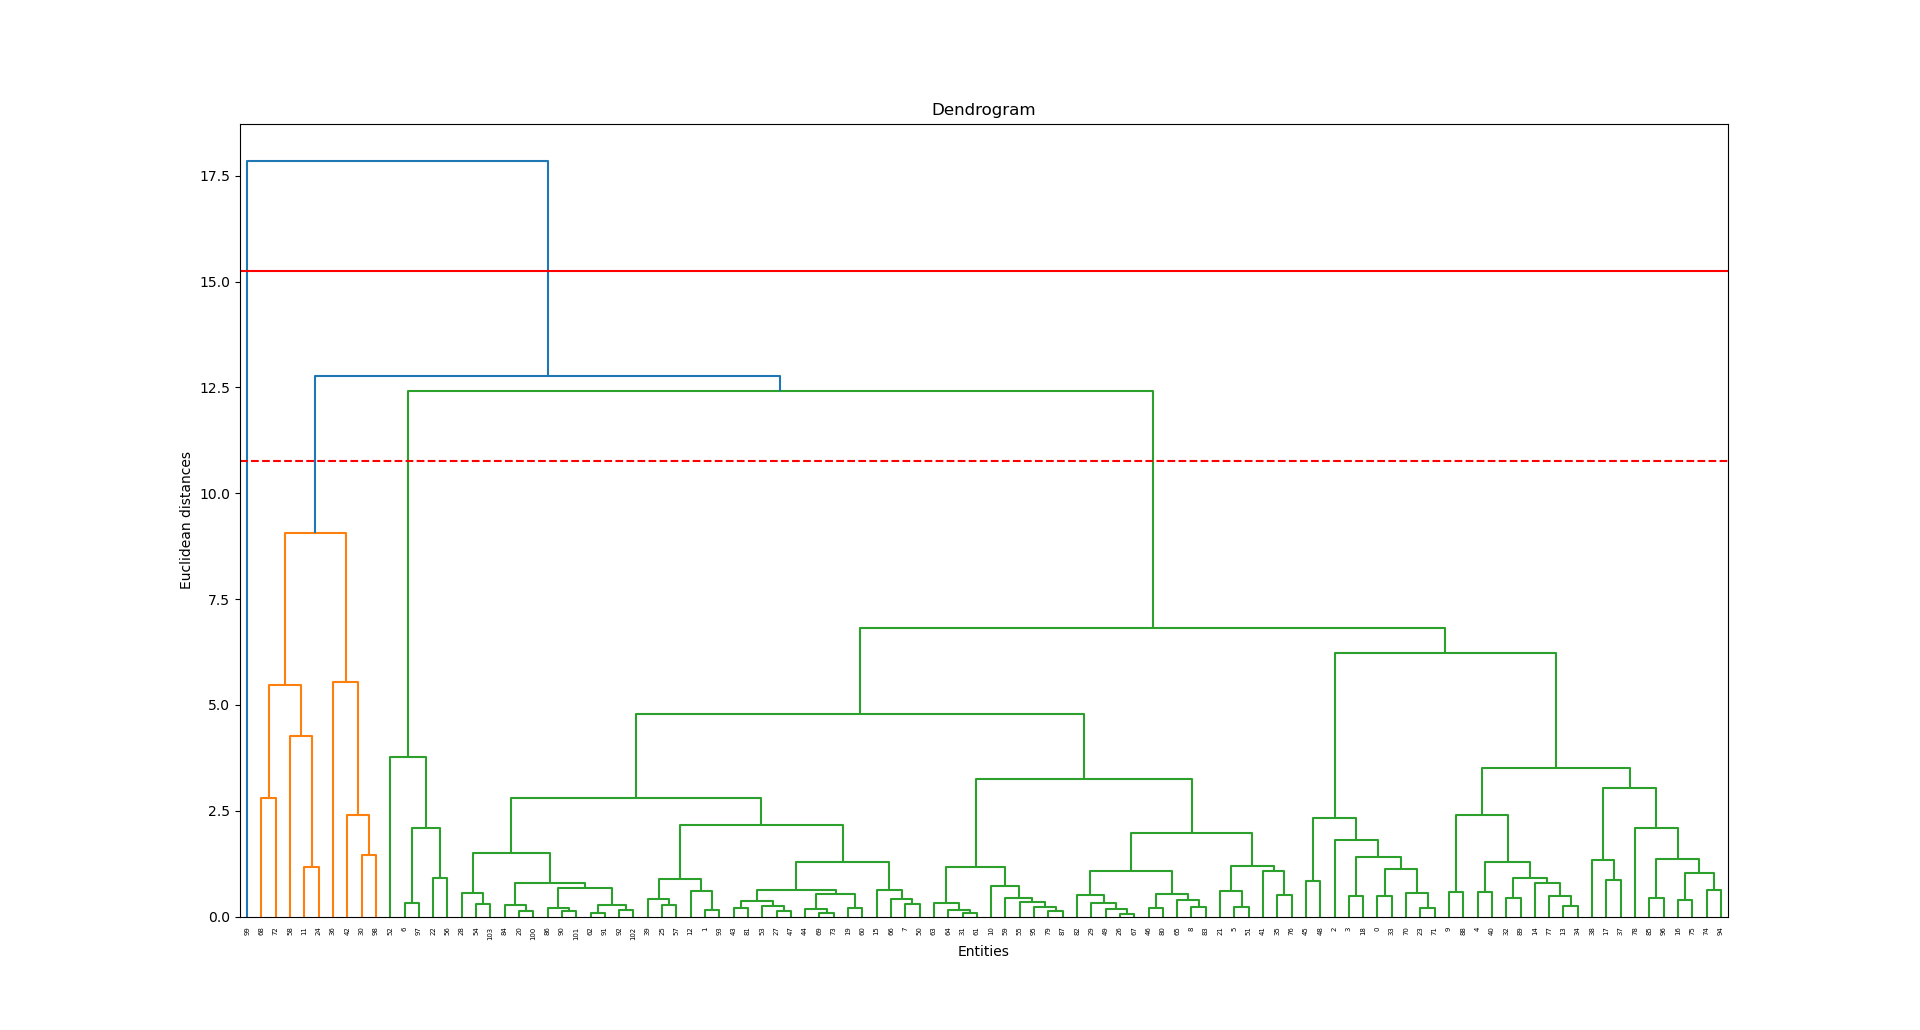
\includegraphics[width=\textwidth]{Figures/Question2/1. Dendrogram.png}
	\caption{Δενδρόγραμμα για προσέγγιση αριθμού clusters στο Agglomerative Clustering}
\end{figure}

Παρατηρούμε ότι το μέση της μεγαλύτερης απόστασης μεταξύ groupings γίνεται εκεί που έχουμε σχεδιάσει την κόκκινη γραμμή. Οπότε η γραμμή αυτή τέμνει τρεις κάθετες γραμμές, οπότε η προσέγγιση του ιδανικού αριθμού clusters που κάναμε οδήγησε σε 3 clusters.

\subsubsection{Αποτελέσματα Agglomerative Clustering με 3 Clusters}

Άρα προχωρώντας τώρα στη διαδικασία του agglomerative clustering με συνολικό αριθμό 3 clusters δημιουργούνται τα εξής clusters:

\begin{itemize}
    \item \textbf{Cluster 1:} Albania, Algeria, Argentina, Armenia, Australia, Bangladesh, Bhutan, Bolivia, Bosnia and Herzegovina, Cape Verde, Chile, Colombia, Costa Rica, Cuba, Dominican Republic, Ecuador, El Salvador, Ethiopia, Fiji, Ghana, Guatemala, Indonesia, Iran, Iraq, Israel, Jamaica, Jordan, Kenya, Kuwait, Libya, Madagascar, Malawi, Malaysia, Mauritania, Mexico, Morocco, Mozambique, Myanmar, Namibia, Nepal, New Zealand, Nigeria, Oman, Pakistan, Panama, Paraguay, Peru, Philippines, Qatar, Rwanda, Saudi Arabia, Senegal, South Africa, Sri Lanka, Thailand, Togo, Trinidad and Tobago, Tunisia, Turkey, Uganda, Uruguay, Vietnam, Zambia, Zimbabwe
    \item \textbf{Cluster 2:} Austria, Bahrain, Belarus, Belgium, Bulgaria, Canada, Croatia, Cyprus, Denmark, Estonia, Finland, France, Greece, Hungary, Iceland, Ireland, Italy, Japan, Kazakhstan, Latvia, Lithuania, Luxembourg, Malta, Mongolia, Norway, Poland, Portugal, Romania, Russia, Serbia, Slovakia, Slovenia, South Korea, Sweden, Switzerland, Ukraine, United Arab Emirates, United Kingdom
    \item \textbf{Cluster 3:} India, United States
\end{itemize}

Τα παραπάνω clusters έχουν τα εξής στατιστικά στοιχεία:

\begin{itemize}
    \item \textbf{Cluster 1:}
        \begin{itemize}
            \item \textbf{Continent:} mean = 0.33, std = 0.87
            \item \textbf{Latitude: }mean = -0.57, std = 0.84
            \item \textbf{Longitude:} mean = -0.04, std = 1.14
            \item \textbf{Average temperature per year:} mean = 0.56, std = 0.62
            \item \textbf{Hospital beds per 1000 people:} mean = -0.51, std = 0.44
            \item \textbf{GDP/Capita:} mean = -0.44, std = 0.56
            \item \textbf{Population:} mean = -0.07, std = 0.38
            \item \textbf{Median age:} mean = -0.57, std = 0.77
            \item \textbf{Cases:} mean = -0.16, std = 0.20
            \item \textbf{Deaths:} mean = -0.15, std = 0.46
            \item \textbf{Positive Ratio:} mean = 0.27, std = 1.19
            \item \textbf{Death Ratio:} mean = -0.14, std = 0.81
            \item \textbf{Tested Ratio:} mean = -0.35, std = 0.38
        \end{itemize}
    \item \textbf{Cluster 2:}
        \begin{itemize}
            \item \textbf{Continent:} mean = -0.63, std = 0.91
            \item \textbf{Latitude:} mean = 0.94, std = 0.37
            \item \textbf{Longitude:} mean = 0.10, std = 0.69
            \item \textbf{Average temperature per year:} mean = -0.95, std = 0.81
            \item \textbf{Hospital beds per 1000 people:} mean = 0.90, std = 1.08
            \item \textbf{GDP/Capita:} mean = 0.70, std = 1.14
            \item \textbf{Population:} mean = -0.18, std = 0.24
            \item \textbf{Median age:} mean = 0.97, std = 0.50
            \item \textbf{Cases:} mean = -0.05, std = 0.37
            \item \textbf{Deaths:} mean = -0.04, std = 0.52
            \item \textbf{Positive Ratio:} mean = -0.45, std = 0.27
            \item \textbf{Death Ratio:} mean = 0.25, std = 1.26
            \item \textbf{Tested Ratio:} mean = 0.58, std = 1.40
        \end{itemize}
    \item \textbf{Cluster 3:} 
        \begin{itemize}
            \item \textbf{Continent:} mean = 1.31, std = 0.38
            \item \textbf{Latitude:} mean = 0.21, std = 0.45
            \item \textbf{Longitude:} mean = -0.46, std = 2.04
            \item \textbf{Average temperature per year:} mean = 0.02, std = 1.22
            \item \textbf{Hospital beds per 1000 people:} mean = -0.59, std = 0.62
            \item \textbf{GDP/Capita:} mean = 0.68, std = 2.02
            \item \textbf{Population:} mean = 5.67, std = 5.18
            \item \textbf{Median age:} mean = 0.05, std = 0.83
            \item \textbf{Cases:} mean = 6.24, std = 4.07
            \item \textbf{Deaths:} mean = 5.48, std = 4.37
            \item \textbf{Positive Ratio:} mean = -0.18, std = 0.18
            \item \textbf{Death Ratio:} mean = -0.08, std = 0.41
            \item \textbf{Tested Ratio:} mean = 0.28, std = 0.96
        \end{itemize}
\end{itemize}

\subsubsection{Αποτελέσματα Agglomerative Clustering με distance threshold ίσο με 7}

Επειδή παρατηρούμε τα παραπάνω αποτελέσματα ότι η μέθοδος εύρεσης αριθμού clusters μέσω δενδρογράμματος οδήγησε σε αποτελέσματα που έχουν πολλές φορές μεγάλη διακύμανση σε στοιχεία όπως τις γεωγραφικές συντεταγμένες και το 'GDP/Capita', καθώς και άλλες, αποφασίσαμε να δοκιμάσουμε διάφορες άλλες τιμές για το distance threshold, έτσι επηρεάζοντας άμεσα τον αριθμό των clusters, με σκοπό να παρατηρήσουμε τα αποτελέσματα και να τα συγκρίνουμε με τα παραπάνω σε επόμενο βήμα, ώστε να καλύψουμε και την περίπτωση της μεθόδου του δενδρογράμματος να μην δώσει την ιδανική τιμή. Από τις δοκιμές μας καταλήξαμε σε τιμή distance threshold ίση με 7.

Γνωρίζουμε πως η εκφώνηση ζητάει το clustering με βάση την επίδοση στην αντιμετώπιση του ίου και όχι με βάση τις τιμές όπως τις γεωγραφικές συντεταγμένες που αναφέρθηκαν παραπάνω ότι έχουν μεγάλη διακύμανση, αλλά θεωρούμε πως οι τιμές αυτές δίνουν μεγάλη έμμεση πληροφορία και ως προς την αντιμετώπιση, εφόσον χώρες κοντά μεταξύ τους έχουν συνήθως πιο μεγάλες ανταλλαγές πληθυσμών και παρόμοια οικονομική κατάσταση, όπως αναφέρθηκε και στην περιγραφή της υλοποίησης του clustering παραπάνω, για αυτό καθιστώντας την επιπλέον δοκιμή χρήσιμη.

Για τη διαδικασία του agglomerative clustering με distance threshold = 7 δημιουργούνται τα εξής clusters:

\begin{itemize}
    \item \textbf{Cluster 1:} Albania, Algeria, Argentina, Armenia, Bosnia and Herzegovina, Chile, Colombia, Libya, Morocco, Paraguay, South Africa, Tunisia, Uruguay
    \item \textbf{Cluster 2:} Bahrain, Cyprus, Denmark, Luxembourg, Malta, United Arab Emirates
    \item \textbf{Cluster 3:} Canada, Finland, Iceland, Ireland, Norway, Sweden, Switzerland
    \item \textbf{Cluster 4:} Australia, Bangladesh, Bhutan, Fiji, Indonesia, Iran, Iraq, Israel, Jordan, Kuwait, Malaysia, Myanmar, Nepal, New Zealand, Oman, Pakistan, Philippines, Qatar, Saudi Arabia, Sri Lanka, Thailand, Turkey, Vietnam
    \item \textbf{Cluster 5:} Japan, Kazakhstan, Mongolia, Russia, South Korea
    \item \textbf{Cluster 6:} Belgium, France, Italy, United Kingdom
    \item \textbf{Cluster 7:} United States
    \item \textbf{Cluster 8:} Cape Verde, Ethiopia, Ghana, Kenya, Madagascar, Malawi, Mauritania, Mozambique, Namibia, Nigeria, Rwanda, Senegal, Togo, Uganda, Zambia, Zimbabwe
    \item \textbf{Cluster 9:} Bolivia, Ecuador, Mexico, Peru
    \item \textbf{Cluster 10:} Austria, Belarus, Bulgaria, Croatia, Estonia, Greece, Hungary, Latvia, Lithuania, Poland, Portugal, Romania, Serbia, Slovakia, Slovenia, Ukraine
    \item \textbf{Cluster 11:} Costa Rica, Cuba, Dominican Republic, El Salvador, Guatemala, Jamaica, Panama, Trinidad and Tobago
    \item \textbf{Cluster 12:} India
\end{itemize}

Τα παραπάνω clusters έχουν τα εξής στατιστικά στοιχεία:

\begin{itemize}
    \item \textbf{Cluster 1:}
        \begin{itemize}
            \item \textbf{Continent:} mean = -0.48, std = 0.43
            \item \textbf{Latitude:} mean = -0.63, std = 1.29
            \item \textbf{Longitude:} mean = -0.58, std = 0.71
            \item \textbf{Average temperature per year:} mean = -0.02, std = 0.68
            \item \textbf{Hospital beds per 1000 people:} mean = -0.18, std = 0.46
            \item \textbf{GDP/Capita:} mean = -0.52, std = 0.19
            \item \textbf{Population:} mean = -0.18, std = 0.15
            \item \textbf{Median age:} mean = -0.03, std = 0.54
            \item \textbf{Cases:} mean = -0.08, std = 0.26
            \item \textbf{Deaths:} mean = -0.05, std = 0.38
            \item \textbf{Positive Ratio:} mean = 0.71, std = 0.82
            \item \textbf{Death Ratio:} mean = -0.03, std = 0.32
            \item \textbf{Tested Ratio:} mean = -0.34, std = 0.19
        \end{itemize}
    \item \textbf{Cluster 2:}
        \begin{itemize}
            \item \textbf{Continent:} mean = -0.38, std = 1.10
            \item \textbf{Latitude:} mean = 0.55, std = 0.50
            \item \textbf{Longitude:} mean = 0.14, std = 0.35
            \item \textbf{Average temperature per year:} mean = 0.11, std = 1.09
            \item \textbf{Hospital beds per 1000 people:} mean = -0.05, std = 0.53
            \item \textbf{GDP/Capita:} mean = 1.42, std = 1.56
            \item \textbf{Population:} mean = -0.32, std = 0.03
            \item \textbf{Median age:} mean = 0.60, std = 0.49
            \item \textbf{Cases:} mean = -0.25, std = 0.05
            \item \textbf{Deaths:} mean = -0.33, std = 0.01
            \item \textbf{Positive Ratio:} mean = -0.65, std = 0.11
            \item \textbf{Death Ratio:} mean = -0.62, std = 0.45
            \item \textbf{Tested Ratio:} mean = 3.29, std = 1.76
        \end{itemize}
    \item \textbf{Cluster 3:} 
        \begin{itemize}
            \item \textbf{Continent:} mean = -0.71, std = 1.01
            \item \textbf{Latitude:} mean = 1.31, std = 0.23
            \item \textbf{Longitude:} mean = -0.50, std = 0.74
            \item \textbf{Average temperature per year:} mean = -1.72, std = 0.45
            \item \textbf{Hospital beds per 1000 people:} mean = 0.00, std = 0.30
            \item \textbf{GDP/Capita:} mean = 2.07, std = 0.69
            \item \textbf{Population:} mean = -0.27, std = 0.09
            \item \textbf{Median age:} mean = 0.89, std = 0.26
            \item \textbf{Cases:} mean = -0.18, std = 0.11
            \item \textbf{Deaths:} mean = -0.22, std = 0.14
            \item \textbf{Positive Ratio:} mean = -0.55, std = 0.11
            \item \textbf{Death Ratio:} mean = 0.60, std = 1.04
            \item \textbf{Tested Ratio:} mean = 0.24, std = 0.26
        \end{itemize}
    \item \textbf{Cluster 4:} 
        \begin{itemize}
            \item \textbf{Continent:} mean = 0.97, std = 0.18
            \item \textbf{Latitude:} mean = -0.28, std = 0.77
            \item \textbf{Longitude:} mean = 1.07, std = 0.69
            \item \textbf{Average temperature per year:} mean = 0.63, std = 0.64
            \item \textbf{Hospital beds per 1000 people:} mean = -0.50, std = 0.37
            \item \textbf{GDP/Capita:} mean = -0.16, std = 0.84
            \item \textbf{Population:} mean = 0.08, std = 0.50
            \item \textbf{Median age:} mean = -0.33, std = 0.56
            \item \textbf{Cases:} mean = -0.14, std = 0.21
            \item \textbf{Deaths:} mean = -0.19, std = 0.25
            \item \textbf{Positive Ratio:} mean = -0.32, std = 0.51
            \item \textbf{Death Ratio:} mean = -0.32, std = 0.73
            \item \textbf{Tested Ratio:} mean = -0.16, std = 0.55
        \end{itemize}
    \item \textbf{Cluster 5:} 
        \begin{itemize}
            \item \textbf{Continent:} mean = 1.04, std = 0.00
            \item \textbf{Latitude:} mean = 0.85, std = 0.40
            \item \textbf{Longitude:} mean = 1.46, std = 0.45
            \item \textbf{Average temperature per year:} mean = -1.39, std = 0.80
            \item \textbf{Hospital beds per 1000 people:} mean = 2.47, std = 1.19
            \item \textbf{GDP/Capita:} mean = 0.04, std = 0.70
            \item \textbf{Population:} mean = 0.16, std = 0.46
            \item \textbf{Median age:} mean = 0.59, std = 1.00
            \item \textbf{Cases:} mean = 0.03, std = 0.59
            \item \textbf{Deaths:} mean = -0.00, std = 0.63
            \item \textbf{Positive Ratio:} mean = -0.56, std = 0.23
            \item \textbf{Death Ratio:} mean = -0.59, std = 0.32
            \item \textbf{Tested Ratio:} mean = -0.15, std = 0.57
        \end{itemize}
    \item \textbf{Cluster 6:} 
        \begin{itemize}
            \item \textbf{Continent:} mean = -1.09, std = 0.00
            \item \textbf{Latitude:} mean = 0.96, std = 0.22
            \item \textbf{Longitude:} mean = -0.26, std = 0.11
            \item \textbf{Average temperature per year:} mean = -0.81, std = 0.34
            \item \textbf{Hospital beds per 1000 people:} mean = 0.47, std = 0.68
            \item \textbf{GDP/Capita:} mean = 1.00, std = 0.25
            \item \textbf{Population:} mean = 0.03, std = 0.19
            \item \textbf{Median age:} mean = 1.17, std = 0.37
            \item \textbf{Cases:} mean = 0.66, std = 0.50
            \item \textbf{Deaths:} mean = 1.09, std = 0.75
            \item \textbf{Positive Ratio:} mean = -0.41, std = 0.07
            \item \textbf{Death Ratio:} mean = 3.14, std = 1.02
            \item \textbf{Tested Ratio:} mean = 0.40, std = 0.52
        \end{itemize}
    \item \textbf{Cluster 7:} 
        \begin{itemize}
            \item \textbf{Continent:} mean = 1.57, std = nan
            \item \textbf{Latitude:} mean = 0.52, std = nan
            \item \textbf{Longitude:} mean = -1.91, std = nan
            \item \textbf{Average temperature per year:} mean = -0.84, std = nan
            \item \textbf{Hospital beds per 1000 people:} mean = -0.14, std = nan
            \item \textbf{GDP/Capita:} mean = 2.11, std = nan
            \item \textbf{Population:} mean = 2.01, std = nan
            \item \textbf{Median age:} mean = 0.64, std = nan
            \item \textbf{Cases:} mean = 9.12, std = nan
            \item \textbf{Deaths:} mean = 8.56, std = nan
            \item \textbf{Positive Ratio:} mean = -0.05, std = nan
            \item \textbf{Death Ratio:} mean = 0.22, std = nan
            \item \textbf{Tested Ratio:} mean = 0.96, std = nan
        \end{itemize}
    \item \textbf{Cluster 8:} 
        \begin{itemize}
            \item \textbf{Continent:} mean = -0.56, std = 0.00
            \item \textbf{Latitude:} mean = -0.94, std = 0.55
            \item \textbf{Longitude:} mean = -0.02, std = 0.36
            \item \textbf{Average temperature per year:} mean = 0.77, std = 0.39
            \item \textbf{Hospital beds per 1000 people:} mean = -0.81, std = 0.30
            \item \textbf{GDP/Capita:} mean = -0.77, std = 0.06
            \item \textbf{Population:} mean = -0.08, std = 0.35
            \item \textbf{Median age:} mean = -1.56, std = 0.26
            \item \textbf{Cases:} mean = -0.27, std = 0.02
            \item \textbf{Deaths:} mean = -0.33, std = 0.01
            \item \textbf{Positive Ratio:} mean = -0.21, std = 0.30
            \item \textbf{Death Ratio:} mean = -0.46, std = 0.39
            \item \textbf{Tested Ratio:} mean = -0.57, std = 0.11
        \end{itemize}
    \item \textbf{Cluster 9:} 
        \begin{itemize}
            \item \textbf{Continent:} mean = 0.37, std = 0.80
            \item \textbf{Latitude:} mean = -0.93, std = 0.67
            \item \textbf{Longitude:} mean = -1.64, std = 0.27
            \item \textbf{Average temperature per year:} mean = 0.36, std = 0.19
            \item \textbf{Hospital beds per 1000 people:} mean = -0.69, std = 0.09
            \item \textbf{GDP/Capita:} mean = -0.54, std = 0.12
            \item \textbf{Population:} mean = 0.00, std = 0.40
            \item \textbf{Median age:} mean = -0.57, std = 0.22
            \item \textbf{Cases:} mean = 0.03, std = 0.29
            \item \textbf{Deaths:} mean = 0.79, std = 1.42
            \item \textbf{Positive Ratio:} mean = 3.58, std = 1.62
            \item \textbf{Death Ratio:} mean = 1.92, std = 1.42
            \item \textbf{Tested Ratio:} mean = -0.56, std = 0.03
        \end{itemize}
    \item \textbf{Cluster 10:} 
        \begin{itemize}
            \item \textbf{Continent:} mean = -1.09, std = 0.00
            \item \textbf{Latitude:} mean = 0.95, std = 0.22
            \item \textbf{Longitude:} mean = 0.01, std = 0.15
            \item \textbf{Average temperature per year:} mean = -0.90, std = 0.38
            \item \textbf{Hospital beds per 1000 people:} mean = 1.25, std = 0.74
            \item \textbf{GDP/Capita:} mean = -0.03, std = 0.48
            \item \textbf{Population:} mean = -0.26, std = 0.09
            \item \textbf{Median age:} mean = 1.20, std = 0.20
            \item \textbf{Cases:} mean = -0.13, std = 0.15
            \item \textbf{Deaths:} mean = -0.15, std = 0.20
            \item \textbf{Positive Ratio:} mean = -0.30, std = 0.32
            \item \textbf{Death Ratio:} mean = -0.05, std = 0.49
            \item \textbf{Tested Ratio:} mean = -0.01, std = 0.30
        \end{itemize}
    \item \textbf{Cluster 11:} 
        \begin{itemize}
            \item \textbf{Continent:} mean = 1.57, std = 0.00
            \item \textbf{Latitude:} mean = -0.34, std = 0.18
            \item \textbf{Longitude:} mean = -1.63, std = 0.16
            \item \textbf{Average temperature per year:} mean = 1.01, std = 0.13
            \item \textbf{Hospital beds per 1000 people:} mean = -0.41, std = 0.57
            \item \textbf{GDP/Capita:} mean = -0.41, std = 0.23
            \item \textbf{Population:} mean = -0.29, std = 0.04
            \item \textbf{Median age:} mean = -0.18, std = 0.76
            \item \textbf{Cases:} mean = -0.25, std = 0.04
            \item \textbf{Deaths:} mean = -0.30, std = 0.04
            \item \textbf{Positive Ratio:} mean = 0.55, std = 1.02
            \item \textbf{Death Ratio:} mean = -0.20, std = 0.36
            \item \textbf{Tested Ratio:} mean = -0.40, std = 0.20
        \end{itemize}
    \item \textbf{Cluster 12:} 
        \begin{itemize}
            \item \textbf{Continent:} mean = 1.04, std = nan
            \item \textbf{Latitude:} mean = -0.11, std = nan
            \item \textbf{Longitude:} mean = 0.98, std = nan
            \item \textbf{Average temperature per year:} mean = 0.89, std = nan
            \item \textbf{Hospital beds per 1000 people:} mean = -1.03, std = nan
            \item \textbf{GDP/Capita:} mean = -0.75, std = nan
            \item \textbf{Population:} mean = 9.33, std = nan
            \item \textbf{Median age:} mean = -0.54, std = nan
            \item \textbf{Cases:} mean = 3.36, std = nan
            \item \textbf{Deaths:} mean = 2.39, std = nan
            \item \textbf{Positive Ratio:} mean = -0.31, std = nan
            \item \textbf{Death Ratio:} mean = -0.37, std = nan
            \item \textbf{Tested Ratio:} mean = -0.40, std = nan
        \end{itemize}
\end{itemize}

\subsubsection{Συμπεράσματα}

Παρατηρώντας τα αποτελέσματα της συσταδοποίησης με αριθμό συστάδων ίσο με τρία παρατηρούμε ότι κάνει πιο high level συσταδοποίηση από την δεύτερη περίπτωση με distance threshold ίσο με 7.

Πιο συγκεκριμένα στην περίπτωση των τριών συστάδων μπορούμε εύκολα να κατηγοριοποιήσουμε τις κλάσεις ως η πρώτη πήγε 'μέτρια' ή δεύτερη πήγε 'καλά' και η τρίτη πήγε 'άσχημα'. Παρατηρούμε όμως ότι πολλές φορές μέσα στις ίδιες τις συστάδες υπάρχει σημαντική διαφοροποίηση στην απόδοση, το οποίο καταλαβαίνουμε από τις τιμές του 'std' στις μετρικές των 'Positive Ratio', 'Death Ratio' και 'Tested Ratio'.

Έτσι ενώ η συσταδοποίηση με τρεις συστάδες αποτελεί ένα πολύ καλό high level approach, στην συσταδοποίηση με distance threshold ίσο με 7, που οδήγησε σε 12 συστάδες έχουμε πιο μεγάλο intracluster similarity για τις σημαντικές αυτές μετρικές που αναφέρθηκαν. Σε αυτή τη περίπτωση όμως υπάρχει ταυτόχρονα μεγαλύτερη ομοιότητα στις υπόλοιπες έμμεσες μετρικές που αναφέρθηκαν, όπως οι γεωγραφικές συντεταγμένες, το οποίο δεν προκαλεί πρόβλημα εφόσον, όπως έχουμε αναφέρει προηγουμένως, και οι μετρικές αυτές παίζουν έμμεσο ρόλο στην αντιμετώπιση του ίου, και παρατηρούμε ότι δεν επηρεάστηκε αρνητιμά το intracluster similarity στις μετρικές που συμβάλουν άμεσα την επίδοση αντιμετώπισης του ιού.

Σχετικά με τις χώρες που ξεχωρίζουν αρνητικά, αναφέρουμε την Αμερική και την Ινδία, που αποτέλεσαν το τρίτο cluster στην συσταδοποίηση με τρεις συστάδες και ξεχωριστά clusters στην συσταδοποίηση με distance threshold ίσο με 7. Οι δύο αυτές χώρες παρουσιάζουν μεγάλη διαφοροποίηση στο 'Population', στα 'Cases' και στα 'Deaths', και προφανώς αυτές που έχουν να κάνουν με την τοποθεσία, αλλά όμοιες μετρικές σχετικά με το 'Positive Ratio' και 'Death Ratio' και 'Hospital beds per 1000 people', το οποίο εξηγεί την συσταδοποίηση τους μαζί στη πρώτη περίπτωση και ξεχωριστά στη δεύτερη περίπτωση, και ας ήταν και οι δύο οι χώρες που ξεχώρισαν για την αρνητική τους αντιμετώπιση του ιού.

Σχετικά με τις χώρες που ξεχωρίζουν θετικά, αναφέρουμε ότι δεν ξεχωρίζουν χώρες στην περίπτωση της συσταδοποίηση με τρεις συστάδες, αλλά αυτές που πήγαν καλά αποτελούν τη δεύτερη συστάδα. Στην περίπτωση συσταδοποίησης με distance threshold ίσο με 7 αποτελούν τη συστάδα 2.

\end{document}
